\documentclass[]{dukedissertation}
%\documentclass[economy,twoside,bind]{dukedissertation}
% Use the second for a single-spaced copy suitable for duplex printing
% and binding.

% Other useful options (there are more options documented in Chapter 2):
%  * draft -- don't actually include images, print a black bar on overful
%             hboxes
%  * MS    -- Format for a Master's Thesis.  No UMI abstract page, some 
%             textual changes to title page.  


% Useful packages for dissertation writing:
\usepackage{amsmath, amssymb, amsfonts, amsthm}
\usepackage{graphicx}
\usepackage{natbib}
\usepackage[absolute]{textpos}
\usepackage{color}
\usepackage{bm}
\usepackage{subfigure}
%\usepackage{g}
\usepackage{mathabx}
\usepackage{multirow}
\usepackage{setspace}
% \usepackage{cite}  % If you include this, hyperlink cites will
                     % break.  It's nice to use this package if your bibstyle
							% sorts entries by order-of-use, rather than
							% alphabetically (as plain does).
							
%Theorem, Lemma, etc. environments
\newtheorem{theorem}{Theorem}%[section]
\newtheorem{lemma}[theorem]{Lemma}
\newtheorem{proposition}[theorem]{Proposition}
\newtheorem{corollary}[theorem]{Corollary}
\newtheorem{result}[theorem]{Result}

% Personal commands and abbreviations.
%Define and personal commands here

%Graphics Path to find your pictures
\graphicspath{{./Pictures/}}


%-----------------------------------------------------------------------------%
% PREAMBLE 
%-----------------------------------------------------------------------------%
\author{Nicolas Di Vara}
\title{Study of time profiles of heavy scintillating crystals}
\supervisor{Marco Paganoni}
\department{Physics} % Appears as Department of \department
% Declare dissertation subject used on UMI abstract page.  List of
% categories: http://dissertations.umi.com/duke/subject_categories.html
%\subject{[Your Subject Here]}

\date{2014} % Anything but the year is ignored.

% Copyright text.  If undefined, default is 'All rights reserved'
% (Example sets the text to a hyperlinked Creative Commons Licence)
\copyrighttext{ All rights reserved except the rights granted by the\\
   \href{http://creativecommons.org/licenses/by-nc/3.0/us/}
        {Creative Commons Attribution-Noncommercial Licence}
}

% Committee Members other than supervisor.  No more than five beyond the
% supervisor allowed.
%\member{[Department Committee Member \#1]}
%\member{[Department Committee Member \#2]}
%\member{[External Committee Member]}
%-----------------------------------------------------------------------------%


%-----------------------------------------------------------------------------%
% HYPERREF: plain black hypertext references for ref's and cite's.
%-----------------------------------------------------------------------------%
\usepackage[pdftex, pdfusetitle, plainpages=false, 
				letterpaper, bookmarks, bookmarksnumbered,
				colorlinks, linkcolor=black, citecolor=black,
	         filecolor=black, urlcolor=black]
				{hyperref}

\begin{document}

%-----------------------------------------------------------------------------%
% TITLE PAGE -- provides UMI abstract title page & copyright if appropriate
%-----------------------------------------------------------------------------%
\maketitle


%\dedication{To AGG}
%
\front

\linespread{1.5}                        %comando per impostare l'interlinea
\pagestyle{empty}

\begin{center}
\par
\vspace{6pt}
%\begin{tabular}{p{5cm}p{5cm}}
\includegraphics[width=.16\textwidth]{../Pictures/Front/logo.png} \hspace{0.5\textwidth}
\includegraphics[width=.16\textwidth]{../Pictures/Front/cern_logo.jpg}\\
%\end{tabular}
\par
\vspace{10pt}
\hrule 
\par
\vspace{18pt}
\par
\begin{large}\textbf{Ph.D. thesis}\\
\par
\vspace{2pt}
\par
December 2014 \\ 
\par
\vspace{8pt}
\par
\end{large} 
\begin{Large}
{\bf Corso di Dottorato in Fisica e Astronomia - Ciclo XXVI}\\
\vspace{-5pt}
Dipartimento di Fisica G.Occhialini\\
\vspace{-10pt}
Universit\`a degli Studi di Milano-Bicocca\\
\vspace{-10pt}
%y\\
%\vspace{-10pt}
%Institut de F\'isica d'Altes Energies\\
\end{Large}
\vspace{80pt}
{\huge \bfseries Study of time profiles} \\
\vspace{6pt}
{\huge \bfseries of heavy scintillating crystals} \\ 
\vspace{6pt}
%{\huge \bfseries at High Luminosity LHC}\\
%\vspace{6pt}
%{\huge \bfseries }
\vspace{80pt} 
\centering
\begin{tabular}{p{10cm}p{1rcm}}
\large Doctoral Student &  \\
\Large \bfseries Nicolas Di Vara & \\
 & \\
 & \\
 & \large Tutor \\
 &\Large \bfseries Prof. Marco Paganoni\\
 &\large Universit\`a degli Studi di Milano-Bicocca\\
 &\large Dipartimento di Fisica G.Occhialini\\
 %& \\
 %& \\
 %& \large External Supervisor \\
 %&\Large \bfseries Dr. Etiennette Auffray\\
 %&\large CERN -- PH-CMX\\
 %& \\
 %& \\
\end{tabular}
\vspace{10pt} \\
\hrule \vspace{6pt}
\large 

\begin{textblock}{1}(11.5,13.5)
\includegraphics[scale=0.7]{../Pictures/Front/Logo_Marie-Curie}
\end{textblock}
\begin{textblock}{1}(3,13.5)
\includegraphics[scale=0.3]{../Pictures/Front/Entervision}
\end{textblock}
\end{center}

}
\abstract

In the field of cancer treatment, particle therapy has recently raised the interest of the community due to the high relative biological effectiveness of charged particles.
In particular they prove to be more effective for targeting radio resistant or inoperable tumours.
Nevertheless different sources of error can worsen the dose delivery profile, such as patient mis positioning, evolution of the tumour/morphology of the patient and imprecision in the treatment plannings, due to fragmentation of the incident beam and range uncertainties.
As a consequence a three-dimensional non invasive imaging technique for ion beam therapy monitoring is required. The attention of the community is thus focused on positron emission tomography (PET).

In particular developments in the field of particle detectors push for the use of time of flight information, that allows to improve the sensitivity by improving the signal to noise ratio (SNR). 
In order to benefit from a significative reduction of the SNR, the target is less than 100 ps FWHM coincidence time resolution for the two detectors.
The standard solution for future PET scanners is to make use of heavy scintillating crystals coupled to Silicon PhotoMultipliers. 

This thesis is devoted to the full characterization of the parameters that influence time resolution in a scintillator/photodetector setup, with particular attention focused on the impact of time profiles of heavy scintillators on the performance.

The first part of the presented work has the objective of describing the fundamental model that governs light production and collection in a PET-like setup.
To this purpose a model based on multi-exponential time profiles has been implemented on an existing framework, widening the scope of usage by evaluating the role of Cerenkov photons produced by low energy radiation.

Moreover in order to properly characterized the operational parameters of a scintillator setup, a comparative analysis of ray tracing softwares has been conducted, namely two packages SLitrani and Geant4. The latter has been chosen to build the simulation framework that allowed to disentangle the various source of resolution degradation.

Finally the work focused on the measurements and evaluation of rise time. Non zero rise time in scintillating systems is given by the different processes characterizing energy deposition inside a crystalline lattice, with utmost relevance of the latest stage of electron hole thermalization. The time scale of this phenomenon is $\sim$ 100 ps and until now has proven to be difficult to estimate due to the intrinsic limitations of detection setups.
Samples of different crystalline species such as CeF$_{3}$, LSO:Ce, LuAG:Ce, LuAG:Pr with different doping concentration are the subject of a time resolved analysis. 
Data taking has been performed in two different conditions: excitation at low energy (36 eV) and a PET-like setup (511 KeV).

The first set of measuremnts has been performed at the VUV beamline at Celia, Bordeaux, with an excitation energy of 36 eV. 
The data show results broadly separable in to two main groups: crystals in the LuAG group, with rise times $>$100 ps, and crystals belonging to the LSO group with rise times $<$50 ps. This is due to the different energy transfer mechanism.

The samples were then measured with a positron source ($^{22}$Na) on a experimental bench composed by a MCP-PMT stop detector and a tagging crystal readout by an amplified SiPM.
Rise time order of magnitude proved to be accessible, though mantaining large uncertainties due to the limited resolution and the long accumulation times.
Nonetheless we showed that Cerenkov photons and deep volume excitations introduce a non negligible contribution to the measured rise time. In particular the samples, excited above the Cerenkov threshold and in the deep volume of the crystal due to the energy of the excitation, showed slower rise times, above 100 ps.
Moreover the influence of Teflon diffusive wrapping have been investigated, showing that opening the extraction cone of the crystals leads to higher rise times due to coupling of multiple reflection modes.

%Nell'ambito oncologico terapeutico, la terapia adronica ha recentemente sollevato l'interesse della comunit\á in virt\ú dell'elevato effetto biologico (RBE) delle particelle cariche.
%In particolare si sono rivelate particolarmente efficaci per la cura di tumori radioresistenti o inoperabili.
%Tuttavia sono molteplici le sorgenti di degradazione del profilo di dose rilasciata: modifica nella posizione del paziente, evoluzione del tumore o dei tessuti, imprecisioni nel piano di trattamento dovute a incertezze nel range calcolato e frammentazione degli ioni pi\'u pesanti.
%Di conseguenza si rivela necessaria l'implementazione di un sistema di imaging tridimensionale non invasivo per il monitoraggio in vivo della terapia. L'attenzione della comunit\á si rivolge in particolare verso la Tomografia a Emissione di Positroni (PET).
%
%In particolare i pi\ú recenti sviluppo nell'ambito dei rivelatori di particelle ha indirizzato verso l'utilizzo della tecnologia time-of-flight (TOF), che consente di migliorare la sensitivit\á migliorando il rapporto segnale rumore (SNR). Al fine di beneficiare di una significativa riduzione del livello di rumore, l'obiettivo \é di raggiungere una risoluzione in coincidenza (CTR) inferiore ai 100 ps FWHM per i due rivelatori.
%La soluzione pi\ú comune per macchine PET vede l'impiego di scintillatori pesanti accoppiati a foto rivelatori, come i Silicon Photo Multiplier. 
%
%Questa tesi si concentra sulla caratterizzazione completa dei parametri che influenzano la risoluzione temporale in un sistema cristallo/foto rivelatore, con attenzione particolare rivolta all'impatto dei profili temporali di fluorescenza degli scintillatori sul rendimento del sistema.
%
%La prima parte del lavoro presentato si pone l'obiettivo di descrivere il modello fondamentale che governa la produzione e la raccolta di luce in un sistema PET. In questo senso \é stato ampliato un modello basato su una produzione di luce multi esponenziale, integrato dallo studio del ruolo dei fotoni Cerenkov nella formazione del segnale.
%
%Inoltre al fine di caratterizzare compiutamente i parametri operazionali di un rivelatore a cristallo scintillante, \é stata inizialmente svolta un'analisi comparativa di software di ray tracing, in particolare SLitrani e Geant4. Quest'ultimo \é stato scelto come software di riferimento per costruire il sistema di simulazioni che ha consentito una completa analisi dei dati sperimentali a dispoisizone.
%
%Infine il lavoro si \é concentrato sulla misura e determinazione del rise time. Un rise time non nullo in un sistema fluorescente \é dato dai differenti processi che caratterizzano la deposizione di energia nel reticolo cristallino, con particolare rivelanza dell'ultimo passaggio, la termalizzazione.
%La scala temporale di questo processo \é di 100 ps e finora si \é dimostrato particolarmente difficile da misurare a causa delle limitazioni sperimentali.
%Campioni di specie cristalline diverse (CeF$_{3}$, LSO:Ce, LuAG:Ce, LuAG:Pr) sono il soggetto di un'analisi ad alta risoluzione temporale. I dati sono stati raccolti in due condizioni di eccitazioni differenti: bassa energia (36 eV) e alta energia (511 KeV).
%
%Il primo gruppo di misure ha avuto luogo presso il fascio AURORE VUV nel centro di ricerca CELIA di Bordeaux, con un'eccitazione di 36 eV. I dati hanno mostrato risultati separabili in due famiglie differenti: per i cristalli appartenenti al gruppo dei Garnet (LuAG) il rise time risulta essere $>100$ ps, per le differenti variazioni del LSO  $<50$ ps. Questo \é dovuto al differente meccanismo di trasferimento di energia.
%
%I campioni sono quindi stati misurati con una sorgente di positroni (Na$^{22}$) su un banco sperimentale composto da un MCP-PMT come rivelatore di stop e un cristallo accoppiato a un SiPM come rivelatore di start.
%Il rise time si \é dimostrato accessibile a una misura sperimentale, mantenendo tuttavia larghe incertezze a causa della risoluzione limitata e dei lunghi tempi di accumulazione, che hanno limitato la raccolta statistica.
%Tuttavia abbiamo potuto mostrare che i fotoni Cerenkov e l'eccitazione nel volume del cristallo introducono una componente non trascurabile nel valore del rise time. In particolare, i campioni, eccitati sopra la soglia Cerenkov e nel volume, hanno mostrato rise time superiori a quelli registrati in VUV ($>100$ ps).
%Inoltre \é stata investigata l'influenza di riflettori diffusivi (e.g. Teflon), mostrando che a causa dell'ampliamento del cono ottico di estrazione dei cristalli il rise time aumenta significativamente.}
\abstract

In the field of cancer treatment, particle therapy has recently raised the interest of the community due to the high relative biological effectiveness of charged particles.
In particular they prove to be more effective for targeting radio resistant or inoperable tumours.
Nevertheless different sources of error can worsen the dose delivery profile, such as patient mis positioning, evolution of the tumour/morphology of the patient and imprecision in the treatment plannings, due to fragmentation of the incident beam and range uncertainties.
As a consequence a three-dimensional non invasive imaging technique for ion beam therapy monitoring is required. The attention of the community is thus focused on positron emission tomography (PET).

In particular developments in the field of particle detectors push for the use of time of flight information, that allows to improve the sensitivity by improving the signal to noise ratio (SNR). 
In order to benefit from a significative reduction of the SNR, the target is less than 100 ps FWHM coincidence time resolution for the two detectors.
The standard solution for future PET scanners is to make use of heavy scintillating crystals coupled to Silicon PhotoMultipliers. 

This thesis is devoted to the full characterization of the parameters that influence time resolution in a scintillator/photodetector setup, with particular attention focused on the impact of time profiles of heavy scintillators on the performance.

The first part of the presented work has the objective of describing the fundamental model that governs light production and collection in a PET-like setup.
To this purpose a model based on multi-exponential time profiles has been implemented on an existing framework, widening the scope of usage by evaluating the role of Cerenkov photons produced by low energy radiation.

Moreover in order to properly characterized the operational parameters of a scintillator setup, a comparative analysis of ray tracing softwares has been conducted, namely two packages SLitrani and Geant4. The latter has been chosen to build the simulation framework that allowed to disentangle the various source of resolution degradation.

Finally the work focused on the measurements and evaluation of rise time. Non zero rise time in scintillating systems is given by the different processes characterizing energy deposition inside a crystalline lattice, with utmost relevance of the latest stage of electron hole thermalization. The time scale of this phenomenon is $\sim$ 100 ps and until now has proven to be difficult to estimate due to the intrinsic limitations of detection setups.
Samples of different crystalline species such as CeF$_{3}$, LSO:Ce, LuAG:Ce, LuAG:Pr with different doping concentration are the subject of a time resolved analysis. 
Data taking has been performed in two different conditions: excitation at low energy (36 eV) and a PET-like setup (511 KeV).

The first set of measuremnts has been performed at the VUV beamline at Celia, Bordeaux, with an excitation energy of 36 eV. 
The data show results broadly separable in to two main groups: crystals in the LuAG group, with rise times $>$100 ps, and crystals belonging to the LSO group with rise times $<$50 ps. This is due to the different energy transfer mechanism.

The samples were then measured with a positron source ($^{22}$Na) on a experimental bench composed by a MCP-PMT stop detector and a tagging crystal readout by an amplified SiPM.
Rise time order of magnitude proved to be accessible, though mantaining large uncertainties due to the limited resolution and the long accumulation times.
Nonetheless we showed that Cerenkov photons and deep volume excitations introduce a non negligible contribution to the measured rise time. In particular the samples, excited above the Cerenkov threshold and in the deep volume of the crystal due to the energy of the excitation, showed slower rise times, above 100 ps.
Moreover the influence of Teflon diffusive wrapping have been investigated, showing that opening the extraction cone of the crystals leads to higher rise times due to coupling of multiple reflection modes.

%Nell'ambito oncologico terapeutico, la terapia adronica ha recentemente sollevato l'interesse della comunit\á in virt\ú dell'elevato effetto biologico (RBE) delle particelle cariche.
%In particolare si sono rivelate particolarmente efficaci per la cura di tumori radioresistenti o inoperabili.
%Tuttavia sono molteplici le sorgenti di degradazione del profilo di dose rilasciata: modifica nella posizione del paziente, evoluzione del tumore o dei tessuti, imprecisioni nel piano di trattamento dovute a incertezze nel range calcolato e frammentazione degli ioni pi\'u pesanti.
%Di conseguenza si rivela necessaria l'implementazione di un sistema di imaging tridimensionale non invasivo per il monitoraggio in vivo della terapia. L'attenzione della comunit\á si rivolge in particolare verso la Tomografia a Emissione di Positroni (PET).
%
%In particolare i pi\ú recenti sviluppo nell'ambito dei rivelatori di particelle ha indirizzato verso l'utilizzo della tecnologia time-of-flight (TOF), che consente di migliorare la sensitivit\á migliorando il rapporto segnale rumore (SNR). Al fine di beneficiare di una significativa riduzione del livello di rumore, l'obiettivo \é di raggiungere una risoluzione in coincidenza (CTR) inferiore ai 100 ps FWHM per i due rivelatori.
%La soluzione pi\ú comune per macchine PET vede l'impiego di scintillatori pesanti accoppiati a foto rivelatori, come i Silicon Photo Multiplier. 
%
%Questa tesi si concentra sulla caratterizzazione completa dei parametri che influenzano la risoluzione temporale in un sistema cristallo/foto rivelatore, con attenzione particolare rivolta all'impatto dei profili temporali di fluorescenza degli scintillatori sul rendimento del sistema.
%
%La prima parte del lavoro presentato si pone l'obiettivo di descrivere il modello fondamentale che governa la produzione e la raccolta di luce in un sistema PET. In questo senso \é stato ampliato un modello basato su una produzione di luce multi esponenziale, integrato dallo studio del ruolo dei fotoni Cerenkov nella formazione del segnale.
%
%Inoltre al fine di caratterizzare compiutamente i parametri operazionali di un rivelatore a cristallo scintillante, \é stata inizialmente svolta un'analisi comparativa di software di ray tracing, in particolare SLitrani e Geant4. Quest'ultimo \é stato scelto come software di riferimento per costruire il sistema di simulazioni che ha consentito una completa analisi dei dati sperimentali a dispoisizone.
%
%Infine il lavoro si \é concentrato sulla misura e determinazione del rise time. Un rise time non nullo in un sistema fluorescente \é dato dai differenti processi che caratterizzano la deposizione di energia nel reticolo cristallino, con particolare rivelanza dell'ultimo passaggio, la termalizzazione.
%La scala temporale di questo processo \é di 100 ps e finora si \é dimostrato particolarmente difficile da misurare a causa delle limitazioni sperimentali.
%Campioni di specie cristalline diverse (CeF$_{3}$, LSO:Ce, LuAG:Ce, LuAG:Pr) sono il soggetto di un'analisi ad alta risoluzione temporale. I dati sono stati raccolti in due condizioni di eccitazioni differenti: bassa energia (36 eV) e alta energia (511 KeV).
%
%Il primo gruppo di misure ha avuto luogo presso il fascio AURORE VUV nel centro di ricerca CELIA di Bordeaux, con un'eccitazione di 36 eV. I dati hanno mostrato risultati separabili in due famiglie differenti: per i cristalli appartenenti al gruppo dei Garnet (LuAG) il rise time risulta essere $>100$ ps, per le differenti variazioni del LSO  $<50$ ps. Questo \é dovuto al differente meccanismo di trasferimento di energia.
%
%I campioni sono quindi stati misurati con una sorgente di positroni (Na$^{22}$) su un banco sperimentale composto da un MCP-PMT come rivelatore di stop e un cristallo accoppiato a un SiPM come rivelatore di start.
%Il rise time si \é dimostrato accessibile a una misura sperimentale, mantenendo tuttavia larghe incertezze a causa della risoluzione limitata e dei lunghi tempi di accumulazione, che hanno limitato la raccolta statistica.
%Tuttavia abbiamo potuto mostrare che i fotoni Cerenkov e l'eccitazione nel volume del cristallo introducono una componente non trascurabile nel valore del rise time. In particolare, i campioni, eccitati sopra la soglia Cerenkov e nel volume, hanno mostrato rise time superiori a quelli registrati in VUV ($>100$ ps).
%Inoltre \é stata investigata l'influenza di riflettori diffusivi (e.g. Teflon), mostrando che a causa dell'ampliamento del cono ottico di estrazione dei cristalli il rise time aumenta significativamente.}
\acknowledgements

\begin{center}
Nothing matter but the quality 

of the affection -

in the end - that has carved the trace in the mind 

\textit{dove sta memoria}

(Ezra Pound, \textit{The Pisan Cantos}, Canto LXXVI)
\end{center}

In every moment of my professional and emotional life the three years spent at CERN will always be a central memory. Every moment, every discussion, every corner will eventually smooth out, but intact will be the eyes and the faces of the people that have helped me. Everyone in his own way, everyone in his own place, everyone carved \textit{dove sta memoria}.

I am grateful to the people that, at some point in my career have believed in me, and I can imagine how difficult it could have been at times. Many thanks to my supervisors, Marco Paganoni, Etiennette Auffray and Paul Lecoq. It has been a pleasure to discuss, argue, agree and disagree and to retain the freedom and respect in this group not only as a value, but as an example.

Everyone at CERN, in that "lab within the lab" that is building 27 has helped me, at some point. Someone helped me out with electronics, someone with crystal theory, someone with a gentle word, or a simple smile. Many thanks then to Stefan, Kristof, Alessio, Benjamin. Thanks to my office mate Mythra, for the discussions on semantics and Indian food and Indian mythology. Thanks to Rosanita, Arno, Pawel, Dominique, Tom, Rita, Gianluca, Giulia, PierPaolo, Farah, Katayoun, Igor. 
Many thanks to Patrick Martin at CELIA, for his helpfulness and old-time courtesy. 
A hug to the guys at the CERN Rugby Club, just to remember that dirt, honour, fall and joy share the same dusty ground.

I would not be writing these confuse paragraphs if it was not for the Entervision project. A shiny example of what Europe could and should be, of the beautiful strength that comes from diversity. Sincere thanks to the Entervision group, at CERN and around: Manjit, Helen, Carlo, Antonios, Joakim, Carlos, Robert, Marco and Marco, Thiago, Ben, Romain, Marie, Frauke, Yuan, Fernando, Manuela. Always remember the beautiful victory at the water and straws contest!

Special thanks to the Ornex Gourmet Club: Pizzi, Amassiro, Cuccia, Raffa. Thanks for the cigarettes, the FIFA matches, the dinners, the laughs.
And thanks to all the friends around that have showed me how important is to be loved. Thanks to Fil, Diana and Rebecca. Thanks to Alessio, Valerio, Tanietta, Gerry and Paola. Special thanks to my cousin Ilias and Krizia, for having me as a Southern man for a few days here and there.

When you leave home, you always feel like an orphan, waiting for a \textit{Rachel} to pick you up. It seems like a shadow line, but it is more like a silent step in a back door garden. I tried to grasp, from a distance, what I could, and all my friends are still there. And I retain this as crafty art work and as an empirical demonstration that love is a daily exercise. Thanks to those Old friends, always ready for a word, for that rare passage of the expat: Morris, Guada and Giorgia, Pagnu, Zuenni, Passo, Marco and Fede, Falco and Lucy, Belci and Angela, Triz, Paul.

And leaving home is also facing the Italian \'etude of stepping out and rediscover. My family is special. It is special for the secular feeling of freedom, for the innate strength that led who forerun me from the dusty roads of the South to the sweaty concrete of the North. A step outside home allows to fully understand the difference between a community bound by love and a society bound by law. Whatever I am, I owe to my family. Thank you Mum, thank you Dad, thank you Mela.

But whatever you discover, stays with you. To find a place and call it home is never easy. Whenever you leave a family, albeit temporarily, it is a struggle of glimpses and silences to find a new one. No one can live on his own, and Fortune sometimes has good calls. One of these calls was to find an incredible group of people, with hearts of builders and eyes of sailors to share this incredible passage of my life. Thanks then to AGG extended and its newer versions. Thanks to Fede, Tolly, Leo, Bengala, Vincent, Anto, Annarella.

Brothers.


}

\tableofcontents 

\begin{savequote}[75mm] 
Nulla facilisi. In vel sem. Morbi id urna in diam dignissim feugiat. Proin molestie tortor eu velit. Aliquam erat volutpat. Nullam ultrices, diam tempus vulputate egestas, eros pede varius leo.
\qauthor{Quoteauthor Lastname} 
\end{savequote}

% COSA MANCA (bilbio, figure, formule ovviamente)
% radioterapia oggi:perche la si fa e quanto
% image reconstruction
% sensitivity
% outline

\chapter{The title of chapter one}

- radiotherapia oggi (vs surgery and chemio) - serve fonte

- serve fonte, ho usato katia parodi

Results of radiotherapy are improved when a high dose of radiation with high biological effectiveness is delivered to the tumour with the least possible dose to the surrounding tissues, especially in the case of critical organs \cite{Linz2011}.
In order to increase the conformity of the dose delivered to the tumour, diverse technologies have been considered and used.
Traditional forms of radiotherapy, X-ray tubes (energy $\sim$ 100 keV) or radioactive isotopes have been replaced by linear accelerators delivering $\sim$ 10 MeV from different directions (e.g. Intensity Modulated Radio Therapy), and provide treatment with photons and electrons.
Though being widely used as a standard in radiation therapy, the effectiveness of conventional electromagnetic radiation is limited by the intrinsic characteristics of interaction with matter.
In particular two aspects disfavours in principle the usability of electromagnetic radiation with respect to ion for tumour targeting: the depth dose profile, which does not allow for an optimal dose deposition to the tumour sparing vital organs
and the inferior biological effectiveness, which is the limiting factor in case of radio resistant tumours.
Heavier charged particles, like protons and ions (He-Ca) have the potentiality to overcome the limits of conventional therapy With respect to this, the scientific community is directing his attention towards possible improvements of ion beam therapy \cite{Amaldi2011}.

- qui citare entervision website

The work outlined in these pages have been sponsored by  The European training network in digital medical imaging for radiotherapy (ENTERVISION) at the European Center of Nuclear Research (CERN). ENTERVISION was established in February 2011 in response to the critical need for reinforcing research in online 3D digital imaging and the training of professionals in order to deliver some of the key elements and building blocks for realizing the vision for early detection and more precise treatment of tumours.

\section{Hadrontherapy}
\subsection{Ion beam therapy}

The first proposition of ion beam therapy was presented in 1946 by R. Wilson \cite{Wilson1946}. The original idea was exploit the physical properties of ion interaction in matter to improve the precision in radiotherapy treatments.  
Making use of the so called Bragg peak, that is using the fact that protons and ions in general deposit a maximum of energy at the end of their trajectory, the treatment could save the surrounding tissue from radiation overdose.
\begin{figure}  
\includegraphics[width=\textwidth]{figures/Chapter_1/conformal_x_rays}
\caption[Short figure name.]{Schematic view of depth-dose distributions of photons and ions. (a) photon
field, (b) spread-out ion beam, (c) depth–dose profiles along the central beam axis \cite{Linz2011}.}
\label{fig:myInlineFigure}}
\end{figure}

The dose deposited by photons, considered as the gold standard for tumour treatment, is maximum close to the beginning of the trajectory in the body and is characterized by an exponential decrease. As a consequence an undesired radiation dose is delivered to healthy tissues around the targeted tumour.

The recent therapeutic interest of ions in the field of radiotherapy relies mainly on their high relative biological effectiveness.
LET (linear energy transfer) has long been viewed as the main parameter to discern the biological effect of different kinds of radiation. It is a measure for the energy deposited by a charged particle traveling through matter. LET is closely related to stopping power and is not a constant value, since it changes along the particle's path (es 10 kEV/um for gamma, 100 kev/um for protons, 1000 kev/um for ions).
When considering ions of different atomic number LET becomes a limited parameter to evaluate the biological effect. In this sense the relative biological effectiveness (RBE) is considered the most accurate quantity, since it is defined as the biological effect of one type of ionizing radiation relative to another, given the same amount of absorbed energy. As the charge of the incident ions increases, so does the probability of severe DNA damage. An elevate RBE in the Bragg peak region has clearly been demonstrated for ions heavier than Helium \cite{Linz2011}.
As a consequence they prove to be more effective for targeting radio resistant or inoperable tumours.

\subsection{Beam delivery}

Ion beams are delivered by either cyclotrons or synchrotrons. In the first case the beam has a fixed energy which is tuned by means of degraders in order to deliver the correct dose profile. In the case of synchrotron the beam is delivered in spills and the energy is varied between spills. In the case of Carbon only synchrotrons can be used.
To deliver the dose to the planned target volume (PTV) different energies are superimposed in order to obtain the so-called spread-out Bragg peak (SOBP). The beam is usually delivered in a passive beam shaping setup or a scanning system. 

Different sources of error can worsen the dose delivery profile, such as patient mis positioning and evolution of the tumour/morphology of the patient. In addition the complex physics of ion interaction leads to  imprecision in the treatment plannings, due to fragmentation of the incident beam and range uncertainties.

Usually treatment planning systems cope with these problems by irradiating a volume larger than the tumour itself, called planning target volume (PTV) which contains the CTV. Complex compensating systems, including x-ray imaging techniques and patient positioning systems, allow to reduce errors in the dose profiles delivered. Treatment plannings of ion therapy relies for example on accurate values of particle range in tissue obtained from Hounsfield unit of computed tomograms, leading to uncertainties of $1-3\%$ in range calculations \cite{Enghardt2004}.
The dose delivered by a ion beam system is much more sensitive to these deviations than the one delivered by a photon beam. Due to the high biological effectiveness of ion beams wrong ranges could lead to dramatic under dosage to the tumour or over dosage to organ at risk surrounding.
As a consequence a three-dimensional non invasive imaging technique for ion beam therapy monitoring is required. Since ions, unlike photons, are stopped completely in the patient volume, technology like portal imaging are not suitable. The attention of the community is thus focused on positron emission tomography (PET), which relies on the peculiar characteristics of $\beta +$ decay.

\subsection{Monitoring of the beam}

Several attempts have already been undertaken to systematically assess the benefit of the PET method for beam monitoring, the principal one being the set up installed at the experimental carbon ion therapy unit at the Gesellschaft fur Schwerionenfroschung Darmstadt (GSI) \cite{Parodi2004}.
Two alternatives can be considered: the use of positron radioactive ions as projectiles for dose delivery or the detection of $\beta +$ activity given bi nuclei fragmentation.
As an example of the first approach it is interesting to consider the effort made at the Heavy Ion Accelerator in Chiba (Japan), where radioactive beams of $^{11}C - ^{10}C$ ions deliver an activity of $10^{3} - 10^{5}$ $Bq Gy^{-1} cm^{-3}$ within the irradiated volume.
Due to the low production rate of secondary radioactive ions, this approach has been only partially successful.
Another possibility is to make use of the $\beta +$ activation given by the fragmentation of stable ions interacting with the tissue.
The radioactivity is a direct product of the irradiation and, although the activity density is rather low (around 600 $Bq Gy^{-1} cm^{-3}$ for protons), this method provides a rather cheaper and feasible solution \cite{Enghardt2004}.
The activity slides very fast under a reasonable threshold for detectability and the most effective solution is an in-beam scanner.
In-beam PET is currently the main method implemented clinically for in situ monitoring of charged hadron radiotherapy\cite{Crespo2007}.

\section{Positron Emission Tomography}
\subsection{Principles}
Positron Emission Tomography (\ac{PET}) has been introduced as a nuclear medicine imaging technique which measures the distribution of a positron-emitting radionuclide (tracer), which is injected into the body on a biologically active molecule. In the case of in-beam PET the activity is present in the body of the patient due to the activation induced by proton interaction.
After the injection, or during the dose delivery, the subject of a \ac{PET} study is placed within the field of view (\ac{FOV}) of a number of detectors capable of registering incident gamma rays. The radionuclide in the radio tracer decays and the resulting positrons subsequently annihilate with electrons after travelling a short distance ($\sim$ 1 mm) within the body. In the case of in-beam PET activation of the tissues guarantees the detectability. Each annihilation produces two $511$ keV photons travelling in opposite directions and these photons may be detected by the detectors surrounding the subject. The detector electronics are linked so that two detection events unambiguously occurring within a certain time window may be called coincident and thus be determined to have come from the same annihilation. These "coincidence events" can be stored in arrays corresponding to projections through the patient and reconstructed using standard tomographic techniques. The resulting images show the tracer distribution throughout the body of the subject. The scheme of a PET scanner is shown in figure \ref{fig:scheme}.
Positron emission tomography relies on the $\beta ^{+}$ decay of a radionuclide.

The nucleus of the radionuclide can convert a proton into a neutron 
\begin{displaymath}
p\rightarrow n + e^{+} + \nu _{e}
\end{displaymath}
As positrons travel through human tissue, they give up their kinetic energy principally by Coulomb interactions with electrons. As the rest mass of the positron is the same as that of the electron, the positrons may undergo large deviations in direction with each Coulomb interaction, and they follow a tortuous path through the tissue as they give up their kinetic energy.

When the positrons reach thermal energies, they start to interact with electrons either by annihilation, which produces two $511$ keV anti-parallel photons, or by the formation of a hydrogen-like orbiting couple called positronium. In its ground-state, positronium has two forms: ortho-positronium, where the spins of the electron and positron are parallel, and para-positronium, where the spins are anti-parallel. Para-positronium again decays by self-annihilation, generating two anti-parallel $511$ keV photons. Ortho-positronium self-annihilates by the emission of three photons. Both forms are susceptible to the pick-off process, where the positron annihilates with another electron. Free annihilation and the pick-off process are responsible for over $80\%$ of the decay events.

\subsection{Image reconstruction}

\subsection{Sources of noise and sensitivity}
In a \ac{PET} scanner, each detector generates a timed pulse when it registers an incident photon. These pulses are then combined in coincidence circuitry, and if the pulses fall within a short time-window, they are deemed to be coincident (see figure).
A coincidence event is assigned to a line of response (\ac{LOR}) joining the two relevant detectors. In this way, positional information is gained from the detected radiation without the need of a physical collimator. This is known as electronic collimation.
When a physical collimator is used, directional information is gained by preventing photons which are not normal or nearly normal to the collimator face from falling on the detector. In electronic collimation, these photons may be detected and used as signal.
Coincidence events in \ac{PET} fall into four categories: true, scattered, random and multiple, as shown in figure . 

True coincidences occur when both photons from an annihilation event are detected by detectors in coincidence, neither photon undergoes any form of interaction prior to detection, and no other event is detected within the coincidence time-window.

A scattered coincidence is one in which at least one of the detected photons has undergone at least one Compton scattering event prior to detection. Since the direction of the photon is changed during the Compton scattering process, it is highly likely that the resulting coincidence event will be assigned to a wrong \ac{LOR}. Scattered coincidences add background to the true coincidence distribution which changes slowly with position, decreasing contrast and causing the isotope concentrations to be overestimated. They also add statistical noise to the signal. The number of scattered events detected depends on the volume and attenuation characteristics of the object being imaged, and on the geometry of the \ac{PET} scanner.

Random coincidences occur when two photons not arising from the same annihilation event are incident on the detectors within the coincidence time window of the system. The number of random coincidences in a given \ac{LOR} is closely linked to the rate of single events measured by the detectors joined by that \ac{LOR} and the rate of random coincidences increase roughly with the square of the activity in the \ac{FOV}. As with scattered events, the number of random coincidences detected also depends on the volume and attenuation characteristics of the object being imaged, and on the geometry of the scanner. The distribution of random coincidences is fairly uniform across the \ac{FOV}, and will cause isotope concentrations to be overestimated if not corrected for. Random coincidences also add statistical noise to the data.

% parte sulla sensitivity che manca

\subsection{TOFPET}

It has been shown that in-beam PET could not provide definitive information to the oncologist when medium to large tumors are involved\cite{Fiedler2006}. This is due to the operative parameters of scanners available on the market, with relatively slow scintillators and tomographs covering small solid angles. A decisive improvement could be given by time-of-flight PET (TOF-PET).

Recent developments in scintillator technology and read out electronics allow to build detectors able to detect the time difference between the moment of detection of the opposed gamma rays in coincidence. 

If we define a LOR between two detectors A and B, the distance between the center of the LOR and the annihilation point is given by

$x = (tb − ta ) · c/2$

where c is the speed of light.
Thus the spatial resolution is proportional to the coincidence time resolution (CTR) of the system.
Scanners available on the market today could deliver a 600 picoseconds time resolution, that translates to a positional uncertainties of 9 cm (FWHM) on the LOR.
The quality of the tomographic image largely benefits from the timing information of a TOFPET scanner, since it reduces considerably  the contribution of Compton scattered photons and from photons from outside the field-of-view (FOV). As a consequence the background from scattered and random coincidence is largely suppressed.
The signal to noise ration (SNR) is thus dramatically improved.
%qua sotto manca la voce in biblio
In the case of in-beam PET this is relevant, since it has been shown (Fiedler et al 2007) that during particle irradiation an considerable amount of activity is transported outside the FOV by metabolic processes. Moreover a high backround signal is typical of carbon ion beams (Pawelke 1997)

A useful and pratical estimation of the gain in signal to noise can be formalized as follows

$G = \frac{SNR_{TOF}}{SNR_{non_TOF}} = \sqrt{\frac{2\cdot D}{c \cdot CTR}}$

where D is the diameter of the volume under examination, c is the speed of light and CTR is the coincidence time resolution. Thus a CTR of 100 ps FWHM translates into a 1.5cm resolution on the position and a SNR gain of 5 (corresponing to a sensitivity gain of about a factor 25) compared to non TOF systems.

\section{Outline of the thesis}
The work presented in this thesis is devoted to the improvement of the operational parameters of TOFPET used in hadrontherapy, with particular respect to fast timing in particle detectors.
\section{From high energy physics to medical applications}

%mancano le citazioni

The present work was hosted by CERN, the European Organisation of Nuclear Research, based in Geneva, Switzerland. 
CERN was established by a formal act in Paris, on 1st of July 1953, as an organisation that ―shall provide for collaboration among European States in nuclear research of a pure scientific and fundamental character, and in research essentially related thereto -.
Thourought its history, CERN provided experimetnal and theoretical tools to study and understand the fundamental forces governing our universe, in a continous effort to improve our understanding of elementary  physics. 

The Large Hadron Collider (LHC), the last effort of scientific community around CERN facility, is the most powerful particle accelerator ever built, expected to accelerate proton beams to an energy of up to 7 TeV maintaining a luminosity of 1034 cm-2s-1. 
The work here presented has been hosted by the CERN section responsible for the development and construciont of the electromagnetic calorimeter (ECAL) of the CMS (Compact Muon Solenoid) experiment.
CMS is a multipurpose detectors used at LHC devoted to the identification and discoveries of new particles and evidence of physics beyond the standard model. It is composed by a 4 T solenoid magnet and several concentric subdetectors that include a tracker, an electromagnetic and a hadronic calorimeter and various layers of muon detectors. 
The ECAL detector was build with the fundamental contribution of the collaboration hosting this thesis: the Crystal Clear Collaboration. It was founded in 1990 as an international academic network of laboratories and industrial partners for the development of scintillating crystal detectors as well as their applications. It comprises experts in crystallography and solid state physics as well as in radiation detection and instrumentation. 
Its first goal was the development of a radiation-hard crystal for the ECAL detector, leading to the development of PbWO4 (PWO) as the material selected for CMS calorimeter. More recently the group has been focusing on the study of new materials for hadronic and electromagnetic calorimeters for future particle accelerators.
In parallel, the collaboration engaged in a effort of technology transfer to other domains exploiting the expertise developed in scintillating detectors. It is quite natural to focus the attention to medical physics, with particular respect to nuclear medicine. As shown in picture () the requirements for detectors used in medical physics and detectors for high energy experiments are similar.

\subsection{Study of time profiles}
- outline vero e proprio
	- panorama pubblicazioni
	- obiettivi
	- strumenti (simulazioni e setups)
	- misure

$x = 1/\alpha$ 

$$\zeta = \frac{1039}{\pi}$$

Fig.~\ref{fig:myFullPageFigure}.


\afterpage{\clearpage}


}

% cristalli in PET, Quenching, optical ( Rayleigh)

\chapter{Scintillating detectors}

In the field of medical applications, the energies of the $\gamma$ photons to be detected are usually of the order of hundreds of keV. In the case of PET scanners the energy of the two back to back photons is 511 KeV.
A simple approach to estimate the parameters of the incoming radiation is to make use of a fluorescent sample coupled to a photo detector. A standard setup would include a heavy scintillator crystal which converts the incoming radiation into visible photons. The following steps of the detection process involve transportation to the entrance window of the photodetector, conversion of the photons into an electric signal and subsequent manipulation of the signal by readout electronics.  

% schema rivelatore anzi no

\section{Interaction of radiation with matter}
In this work we are mainly concerned with the interaction of $\gamma$ radiation with matter, thus focusing our attention on the three existing mechanisms: photo electric interaction, Compton interaction and pair production.
Moreover electrons produced by ionizing interactions can polarize the medium, giving origin to the Cerenkov effect and producing visible photons, which can be of foremost importance in the case of timing application.

\subsection{Photoelectric effect}

In the case of the photoelectric effect an electron from an atom is freed upon absorption of the incoming photon (see figure \ref{fig:photo_electric}):
\begin{equation}
\gamma + atom \rightarrow e^{-} + atom
\end{equation}
Due to conservation of momentum and energy this phenomenon does not occur with free electrons. 
The gamma energy trasnferred to the electron equals the binding energy of the electron itself minus its resulting kinetic energy $E_{eˆ{-}}$ 
\begin{equation}
E_{e^{-}} = E_{\gamma} - E_{b}
\end{equation}
The photoelectric effect is predominant at low energies (E $\geq 100$ KeV) and favours tightly bound K-shell electrons. An approximation of the photo electric cross section is given by
\begin{equation}
\sigma _{pe} \propto \frac{Zˆ{n}}{E_{\gamma}^{3.5}}
\end{equation}
The vacancy created can be filled through capture of bound or free electrons, eventually generating characteristics X-rays.  

\begin{figure}
\centering
\includegraphics[width=7cm]{../Pictures/Chapter_2/photo_el_2}
\caption[Photo electric effect]{Phenomenology of the photo electric effect}
\label{fig:photo_electric}
\end{figure}
\newpage
\subsection{Compton scattering}

Compton scattering is the inelastic scattering of the incoming photon with a weakly bound electron in the material (see figure \ref{fig:compton}):
\begin{equation}
\gamma + atom \rightarrow (\gamma ') + e^{-} + atom^{*}
\end{equation}
Contrary to the photoelectric effect, this only concerns quasi-free electrons of the material. 
The photon transfers part of its energy to the electron, which is freed from its shell.
Applying conservation of energy and momentum it is possible to derive the energy of the scattered gamma as well as the direction and energy of the freed electron.
\begin{equation}
E_{\gamma '} = \frac{E_{\gamma}}{1+\frac{E_{\gamma}}{m_{e}c^{2}}(1-cos\theta)}
\end{equation}
The angular distribution can be described by the Klein-Nishina formula. It can be noted that forward scattering direction are favoured as the incoming photon energy increases
\begin{equation}
\frac{d\sigma _{cpt}}{d\omega} = Z \cdot \frac{e^{2}}{4\pi \epsilon _{0} m_{e} c^{2}} \cdot \frac{1}{2} \cdot \frac{E'_{\gamma}}{E_{\gamma}} \left( 1 - \frac{E'_{\gamma}}{E_{\gamma}} \cdot sin^{2}\theta + \left[ \frac{E'_{\gamma}}{E_{\gamma}} ^{2} \right] \right)
\end{equation}
The total cross section can be computed by integrating the differential cross section over the angle, with $\epsilon = h\nu / mc^{2}$ and $r_{e} = h/mc$.
\begin{equation}
\sigma _{KN} = 2\pi r_{e}^{2} \left{ \frac{1+\epsilon}{\epsilon ^{2}} \left[ \frac{2(1+\epsilon)}{1 + 2\epsilon} - \frac{ln(1+2\epsilon)}{\epsilon}\right] + \frac{ln(1+2\epsilon)}{2\epsilon}-\frac{1+3\epsilon}{(1+2\epsilon)^{2}}\right]
\end{equation}
\begin{figure}
\centering
\includegraphics[width=7cm]{../Pictures/Chapter_2/259px-Compton-scattering.pdf}
\caption[Compton scattering]{Phenomenology of Compton scattering}
\label{fig:compton}
\end{figure}

\subsection{Pair production}

If the energy of the gamma exceeds $2m_{e}c^{2} = 1.02$ MeV, the impinging photons can also be converted into an electron-positron pair. The cross-section of the pair production is given at low energies (thus low screening) by
\begin{equation}
\sigma _{pair} = 4\alpha r_{e}^{2} Z^{2} \left( \frac{7}{9}ln2\frac{E}{m_{e}c^{2}} - \frac{109}{54}\right)
\end{equation}
The cross section is very low compared to that of photoelectric and Compton effect until the energy of the $\gamma$ approaches several electron Volts. Thus for the energies involved in medical applications pair production can be neglected.
The measuredcross section for the processes considered is shown in \ref{fig:cross_section} for Lead. 

\begin{figure}
\centering
\includegraphics[width=9cm]{../Pictures/Chapter_2/sigma_gamma.pdf}
\caption[$\gamma$ cross section]{Cross section for the different processes in lead}
\label{fig:cross_section}
\end{figure}
\newpage
\section{The scintillation mechanism}

As a general idea the scintillation process can be considered as the conversion of the energy of an incident $\gamma$ quantum or particle into a certain number of low energy photons \cite{Rodnyi1997}. In a way it can be therefore defined as a wavelentgh shifting process \cite{Lecoq2006}.

\begin{figure}
\centering
\includegraphics[width=12cm]{../Pictures/Chapter_2/drawing_2.pdf}
\caption[Energy deposition in scintillator]{Chain of energy deposition processes in crystals}
\label{fig:lecoq_easy}
\end{figure}

After a ionization event, generated by the mechanisms presented above in the case of a $\gamma$ interaction, the scintillator relaxes towards a new equilibrium. This process is characterized by a multitude of sub processes, that can be depicted by band diagrams as the one in figure \ref{fig:lecoq_easy}.
As long as the energy of the particles is high enough, it is transferred to secondary particles of lower energy, creating an electromagnetic cascade.
A crystal is an ordered ensemble of atoms, and the electrons in the KeV range start to couple with electrons and atoms of the lattice. As a result of their interaction with electronic states of the material, couples of electrons and relative vacancies are created. The electron hole pairs migrate in the lattice above and below the ionization threshold until they are trapped by a defect or recombine on a luminescent center. Alternatively they cool down by coupling to the lattice vibrations until they reach the top of the valence band (hole) or the bottom of the conduction band (electron). They can also form loosely bound structures called exciton, with en energy slightly smaller than the bandgap energy.
The scintillator itself must contain luminescent centers, either intrinsic or extrinsic (doping ions). These molecular systems in the lattice present characteristic radiative transitions between excited states.
Recombination brings the release of optical photons, at characteristic wavelengths.
%
%The scintillation process can therefore be represented as the sequence of the following stages\cite{Rodnyi1997}: 
%
%\begin{itemize}
%\item Absorption of ionizing radiation and creation of primary e-h pairs
%\item Relaxation of primary e-h pairs with production of secondary e-h pairs, plasmons, photons, etc.
%\item Thermalization of low energy e-h pairs down to the band gap energy $E_{g}$
%\item Energy transfer form the e-h pairs to the luminescence centers
%\item Emission of scintillation photons
%\end{itemize}

\subsection{Creation of electron hole pairs}

To analyze more in depth the mechanisms of the scintillation, we can consider an intermediate energy $\gamma$ ray ( $\sim 500$ KeV) interacting with the scintillator material. In this case the photoelectric effect is dominant. Thus it will produce a hole in a inner shell (usually K shell) and a free or quasifree electron.
\begin{equation}
A + h\nu \rightarrow A^{+} + e
\end{equation}
The energy of the primary electron will be $h\nu - E_{k}$ where $E_{k}$ is the K level energy. The relaxation then happens differently for electrons and holes. 

The ionized atom ($A^{+}$) can relax either radiatively, thus emitting a photon, or nonradiatively, generating a secondary electron. This is know as the Auger effect. Thereafter a cascade of both radiative and nonradiative processes takes place.
The Auger electron and the primary electron begin a proces of electron-electron scattering or phonon emission. In the case of a radiative emission, the soft x-ray photon emitted may be absorbed producing a new deep hole and free electron. 

The electron on the other hand will ionize an atom
\begin{equation}
A + e \rightarrow A^{+} + 2e
\end{equation}
The two undistiguishable electrons will undergo a number of other ionization processes, resulting in an avalanche of secondary electrons and holes. At some point the secondary products of these processes are not able to ionize the medium anymore.
A fast electron can in principle interact also with valence electrons of the medium, producing collective oscillations known as plasmons. Plasmons behave as quasiparticles, with an energy of $\sim 10$ eV and can decay into e-h pairs.

This ensemble of avalanche processes continues until the generated secondaries are not able to create further ionization. At this point electrons and holes start to interact with the vibrations of the lattice in a stage called thermalization, via different mechanisms of electron-phonon interaction. 
 As a consequence, at the end of this chain of de-excitation processes, low energy electronic excitations are present: electrons in the conduction band, holes in the valence band, valence excitons, core excitons.
 
\subsection{Intrinsic luminescence}

\begin{figure}
\centering
\includegraphics[width=12cm]{../Pictures/Chapter_2/traps.pdf}
\caption[Electron hole recombination]{Different processes for electron hole recombination}
\label{fig:traps}
\end{figure}
Electron and holes have several ways to recombine after thermalization and give rise to scintillation photons.
The simplest emission process is direct recombination
\begin{equation}
e + h \rightarrow h\nu
\end{equation}
Recombination can more effectively take place when the energy of the electron and hole has decreased, so that they form an exciton. 
However the various impurities and lattice defects play a very important role in the scintillation process. Thermalized carriers can be bound in some places of the lattice where atom or defects are localized. 
For example many ionic crystals shows phenomena of localization of the valence hole in the lattice, known as self-trapping. This structure appears when a thermalized hole localizes an anion, polarizing the environment. As a result the hole can be shared between two neighbouring ions forming a $V_{k}$ center, and the hole is defined as self-trapped hole. For high energy excitation direct creation of valence exciton is unlikely, so $V_{k}$ centers usually capture free electrons. From subsequent de excitation they can emit photons, thus giving rise to the excitonic luminescence.
\begin{equation} 
e + h \rightarrow ex \rightarrow h\nu
\end{equation}

\subsection{Core to valence transitions}

If the core bands of the scintillator lie below the Ager threshold, the most favoured transitions involve holes in the valence band and electron in the conduction band. Nevertheless some systems present the so-called cross luminescence. This phenomenon implies a direct core to valence transition, due to the fact that holes in uppermost core bands can not de excite non radiatively \cite{Lecoq2006}. 

A notable example of core to valence transition is $BaF_{2}$. In this system a $Ba^{2+}$ $5p$ core hole is above the Auger threshold and hence Auger effect does not occur. They can recombine directly with electrons from the valence band, in most of the cases radiatively.
This leads to a very fast luminescence given by recombination of the core hole, while the primary electron de excitation is more complex thus leading to a slower component.

\begin{figure}
\centering
\includegraphics[width=8cm]{../Pictures/Chapter_2/core_to_valence.pdf}
\caption[Core to valence luminescence]{Direct luminescence (left) versus cross to valence luminescence (right)}
\label{fig:CTV}
\end{figure}
 

\subsection{Extrinsic luminescence}

Most of the scintillator samples used in this work are extrinsic, that is doped with activation centers that can enhance the intrinsic scintillation properties presented above by favouring direct recombination.
Rare earth ions doping, for example, is largely used in scintillator technology because of the parity and spin-allowed transition $4f^{n-1}5d\rightarrow 4f^{n}$. 
Extrinsic scintillators usually present different luminscent mechanisms driven by activated sites \cite{Lecoq2006}:
\begin{itemize}
\item $e + h + A \rightarrow ex + A \rightarrow A^{*} \rightarrow A + h\nu$
\item $e + h + A \rightarrow A^{1+} + e \rightarrow A^{*} \rightarrow A + h\nu$
\item $e + h + A \rightarrow (A^{1-})^{*} + h \rightarrow A + h\nu$
\item $A \rightarrow A^{*} \rightarrow A + h\nu$
\end{itemize}
In the first case the insertion of dopants is able to sufficiently quench the exciton luminescence so that excitation of radiative centers results form a transfer from excited matrix states.
A competing process is the direct capture of free thermalized carriers by luminescent center, in the case of electrons or holes.
In heavy doped or self-activated crystals ($CeF_{3}$) direct excitation by ionizing radiation is possible.

%QUI MANCA QUALCOSA!

\subsection{Quenching phenomena}
TO DO
% thermal, concentration, trapping Chapter3 Lecoq
\section{Operational parameters}
\subsection{Light yield}
One of the feature commonly required of a scintillator is to have a high light yield, that is to be an efficient converter of radiation to visible light.
In this case the relative light output of the scintillator, $L_{R}$, can be considered the significant quantity. It is defined as the number of emitted photons per unit of absorbed energy \cite{Rodnyi1997}
\begin{equation}
L_{R} = \frac{N_{ph}}{E_{\gamma}}
\end{equation}
The number of produced e-h pairs $N_{eh}$ depends on the average energy needed for the creation of a low energy e-h pair, $\chi _{eh}$. This value depends on the type of lattice and band gap of the material, with a numerical coefficient $\beta$
\begin{equation}
\chi _{eh} = \beta \cdot  E_{g}
\end{equation}
If $\alpha$ is the average number of scintillation photons produced by a single e-h pair, the light output is
\begin{equation}
L_{r} = \frac{\alpha \cdot N_{eh}}{E_{\gamma}} = \frac{\alpha}{\chi _{eh}} = \frac{\alpha}{\beta \cdot E_{g}}
\end{equation}
The coefficient $\alpha$ depends on the transport efficiency of the e-h pairs to the luminescence center and the conversion efficiency of the center itself.

\subsection{Optical properties and light transport}
% MANCA QUALCOSA!
TO DO
\subsection{Energy resolution and nonproportionality}
In the case of $\gamma$ spectroscopy it is necessary to discriminate quanta with different energy.
For scintillation detector this fundamental property is characterized by the energy resolution $R$, defined as $\Delta E/E$ (in $\%$) where $\Delta E$ is the full width at half maximum (FWHM) at pulse height $E$.
It depends on the characteristics of the scintillator, i.e. materials, size and defects as well as the coupling with the photo detector and the parameters of the photo detectors itself. Statistical fluctuations at any step of the detector chain, from dynode multiplication to photo cathode efficiency in the case of a PMT can worsen the resolution at the peak. 
Thus energy resolution can be defined as \cite{Rodnyi1997}
\begin{equation}
R^{2} = R_{S}^{2} + R_{PM}^{2} = R_{S}^{2} + \frac{\delta}{E_{\gamma}}
\end{equation}
where $R_{S}$ and $R_{PM}$ are, respectively, the scintillator and photomultiplier contributions and $\delta$ includes photo electron statistics.
It is possible to further decompose the scintillator resolution $R_{S}$ to take into account the factors depending on the type of scintillator used. In particular it is useful to introduce a term for the transfer efficiency of the optical photons $R_{S}$, a term for inhomogeneity $R_{i}$ and a term for nonproportionality $R_{n}$
\begin{equation}
R_{S}^{2} = R_{t}^{2} + R_{i}^{2} + R_{n}^{2}
\end{equation}
The interest lies in the fact that the two terms, for inhomogeneity and nonproportionality, account for the intrinsic resolution of the crystal.
Inhomogeneity arise from possible imperfections of the scintillator, such as local variations in the concentration of the dopant or optical defects.

Non proportionality arise when scintillators show deviation from stability of excitation spectrum, that is when linearity between energy of the excitation and relative light output is not preserved. This is particularly important for low energy excitation, since scintillation phenomena occur mainly on the surface. Non proportionality is caused by the statistical nature of the creation of secondary electrons and photons and contribute to worsen the resolution.

\subsection{Cerenkov effect}
Cerenkov radiation brings important information both in high energy physics and time resolved PET.
Cerenkov radiation occurs when a charged particle passes through a dieletric medium at a speed greater than the phase velocity of light in that medium.
The phase velocity of light in a medium of refractive index $n > 1$ is
\begin{equation}
v_{p} = \frac{c}{n}
\end{equation}
A charged particle can travel faster than the speed of light if, given its velocity $v_{p}$ 
\begin{equation}
\frac{c}{n} < v_{p} < c
\end{equation}
This translates to the following condition for the $\beta$ coefficient of the particle
\begin{equation}
\beta = \frac{v_{p}}{c} > \frac{1}{n}
\end{equation}
For a particle of a given mass thus the energy threshold is
\begin{equation}
K_{thr} = mc^{2}\left( \frac{\sqrt {n^{2}-1}}{n} - 1 \right)
\label{eq:thr}
\end{equation}
The phenomenology of Cerenkov effect can be explained considering the polarization of the medium caused by a charged particle traversing it.
Below the Cerenkov threshold the dipoles surrounding are symmetrically arranged around the path. As the particle crosses the threshold it travels faster than the speed at which it interacts with the dipoles. This symmetry breaking leads to a non-vanishing dipole moment and thus to the formation of a wave front.

\begin{figure}
\centering
\includegraphics[width=9cm]{../Pictures/Chapter_2/cerenkov.pdf}
\caption[Cerenkov effect]{Phenomenology of Cerenkov effect}
\label{fig:cerenkov}
\end{figure}

Cerenkov photons are emitted at a characteristic angle in the forward direction, obtained via simple geometrical considerations. The distance traveled by the charged particle in a time $t$ is $t\cdot \beta \cdot c$ whereas the distance along which the photon propagates is $t\cdot c /n$ as shown in figure \ref{fig:cone}.
Therefore the characteristic angle at which photons are emitted can be calculated as
\begin{equation}
cos(\theta _{C}) = \frac{t c/n}{t \beta c} = \frac{1}{n\beta}
\end{equation}
As will be shown in the next chapter, the direction of emission retains a primary interest in the field of particle identification, while it has a negligible impact on timing measurement in PET scanners. It is worth to be noted that the Cerenkov photons are emitted promptly, taking a relevant share of the first incoming photons.  
\begin{figure}
\centering
\includegraphics[width=9cm]{../Pictures/Chapter_2/cone.pdf}
\caption[Cerenkov emission cone]{Sketch of the Cerenkvo emission cone}
\label{fig:cone}
\end{figure}
It is useful to consider the number of emitted photons per unit length by a charged particle as a function of the wavelength
\begin{equation}
\frac{dN}{d\lambda dx} = \frac{2\pi z^{2}\alpha}{\lambda ^{2}}\left( 1 - \frac{1}{\beta ^{2}n^{2}(\lambda)} \right)
\end{equation}
Neglecting dispersion in the medium, and integrating over an appropriate interval of wavelengths we obtain that the photons are emitted mostly in the UV range.
\begin{equation}
\frac{dN}{dx} = 2\pi z^{2} \alpha \left( 1-\frac{1}{\beta ^{2} n^{2} (\lambda)}\right) \int _{\lambda _{1}} ^{\lambda _{2}} \frac{d\lambda}{\lambda ^{2}}  = 2\pi z^{2}\alpha sin^{2}\theta _{C} \left( \frac{1}{\lambda _{1}}-\frac{1}{\lambda _{2}}\right)
\label{eq:number}
\end{equation}

A simple calculation shows that, even at the low energies that characterize a PET exam (511 KeV), a non negligible number of Cerenkov photons is produced.
As an example, it is interesting to consider the case of the most popoluar crystal for PET detectors, Lu$_{2}$SiO$_{5}$:Ce (LSO) with a density $\rho _{LSO}$ = 7.48 g/cm$^{3}$ and a refractive index of 1.82 \cite{jellison2012}.
Given the K-shell binding energy of the electron (63 KeV \cite{xdata2009}), we can estimate, with the help of formula  \ref{eq:thr}, the energy threshold for Cerenkov production for electrons at 448 KeV.
If we then consider a freed electron from the K-shell and its average range in LSO (265 $\mu$m \cite{nist2005}), we can make use of formula \ref{eq:number}, given that
\begin{equation}
sin ^{2}(\theta _{c}) = 1 - \frac{1}{n^{2}\beta ^{2}} = 0.58
\end{equation}
The number of optical photons produced in the wavelength range 180 - 800 nm is $\sim$ 40.


\section{Most common scintillation processes}
The main crystal species used in this study will be briefly presented in this section, in particular with respect to the scintillation mechanism. Light yield and time profiles will be more deeply analyzed in the next chapters.
% magari puoi anticipare due cose sulle terre rare?
\begin{itemize}
\item \textbf{Lutetium Oxiorthosilicate}: Lutetium oxyorthosilicate (LSO) is a widely used crystal for PET detection and high energy phisics. The crystal structure of Lu$_{2}$Si0$_{5}$:Ce the Lu atoms occupy two equally-populated, crystallographically independent sites, and the Cerium doping atom is assumed to substitute for the Lutetium atom \cite{Naud1996}.
The 5d level is split by the crystal field of the host lattice into 3 sublevels, and the 4f ground state is split by the spin-orbit interaction into two levels.
The luminescence of LSO is due to parity-allowed electric dipole transitions from the lowest 5d sublevel to the split 4f ground state, with emission band at 410 nm.
Due to the high density (7.4 g/cm$^{3}$), very fast emission ($\sym$ 40 ns) and high light yield ($>$40000 photons/MeV) is considered to be on the most important crystals for calorimetry.
\item \textbf{Lutetium Aluminum Garnet}: Lutetium Aluminum Garnet (Al$_{5}$Lu$_{3}$O$_{12}$) has been recently proposed as a candidate for future calorimetry experiment\cite{Kris2013}, for the high density (6.73 g/cm$^{3}$) and fast emission profile of the main components ($<$ 60 ps).
LuAG crystals present relevant intrinsic and extrinsic scintillator characteristics.
The intrinsic scintillation of LuAG comes from processes related to self trapped exciton de excitation. Indeed in case of strong electron hole coupling to the lattice a carrier can be trapped in its own field.
STEs in LuAG lead to absorption band at 7.1 and 7.3 eV and emission upon recombination at 5 eV.
STEs may also localise around Lu$_{Al}^{3+}$ defects and give rise to emission at 3.3 eV.
This recombination mechanisms are very slow, usually $\sym$ 2 $\mu$s and for this reason the LuAG lattice is often doped, as the case of LSO with a rare earth activator (Yb, Pr, Ce).
In particular we will consider the case of Cerium and Praseodymium doping.
The case of Cerium doping is similar to the LSO case, with an emission band peaking at 520
nm that corresponds to the Ce$^{3+}$ 5d$\rightarrow$4f transitions.
In the case pf Praseodymium doping, apart from the excitonic luminescence, two bands are present, corresponding to the Pr$^{3+}$ 4f5d$\rightarrow$4f$^{2}$ and 4f$^{2}\rightarrow$4f$^{2}$ contained respectively in the 285-450 nm band and 450-880 nm band \cite{Drozdowski2008}. For calorimetry application only the first is relevant. 
\item \textbf{Cerium Fluoride}:
\item \textbf{Bismuth Germanate}: Bismuth Germanate (Bi$_{4}$Ge$_{3}$0$_{12}$), or BGO, is been considered for many years the gold standard for radiation detection, in nuclear medicine and high energy physics, because of its high density (7.13 g/cm$\^{3}$), high scntillation output ($>$20000 photons/MeV) and relatively fast emission (two components, main one $\sym$300 ns).
BGO is an intrinsic scintillator, that is no dopant is added. The observed fluorescence is assigned to $^{3}$P$_{1}\rightarrow ^{1}$S$_{0}$ transitions of Bi3$^{+}$, with broad emission band at 490 nm \cite{Weber1996}.
\end{itemize}}
% citazioni, immagini

\chapter{Photo detectors}
After the scintillation phase in the crystal, visible photons are generated and coupled to a photodetector. At this stage the photodetector generates an eletric signal related to the photon rate, by generating free electrons in vacuum or electron-hole pairs in a semiconductor.

As they are used as fundamental components of the experimental apparatus, the vacuum photodetector technology and the solid state technology will be presented.
Vacuum photodetectors are characterized by the production of free electrons in an external photocathode by photoelectric interaction. The produced electrons undergo acceleration in a focused electric field and are multiplied by secondary interaction before being transfered to the read out circuitry. Photo multiplier tubes (PMT) and micro channel plates tubes  (MCP-PMT) are prominent examples of vacuum technology.
  
In the case of solid state photo detectors, photons interact directly in the bulk material, where electron-hole pairs are produced. The pairs are then accelerated in the electric field and multiplied by ionization in the semiconductor itself. In the work presented here, Silicon photo multipliers (SiPM) are used as representative of this kind of detector.     

\section{Photo multiplier tubes}

Photo multiplier tubes are largely used vacuum photo detection devices and have been diffusively discussed in literature \cite{Knoll2000}. 
\begin{figure}[htbp]
\begin{center}
\includegraphics[width=12cm]{../Pictures/Chapter_3/PMT.png}
\end{center}
\caption[PMT schematics]{Schematics of a Photo-Multiplier Tube \cite{Hama2006}.}
\label{fig:PMT_schematics}
\end{figure}
In figure \ref{fig:PMT_schematics} the main elements of a photo multiplier tube are sketched:
\begin{itemize}
\item a photocathode, which converts visible photons into an electron flux
\item an electron-optical input system which focuses and accelerates the electron flux
\item an electron multiplier consisting of a series of secondary emission electrodes (dynodes)
\item an anode, which collects the electron flux and supplies the output signal
\end{itemize}
Photoemission is due to a fraction of the incident visible photons that transfer enough energy to the electrons of the photo cathode to extract them.
Then the focusing system allows the freed electrons to reach the first dynode, i.e. the first multiplication stage. The electrons are accelerated and focused by eletric field between the dynodes and the required potential gradient is usually guaranteed by a voltage divider.

%foto divider

\subsection{Properties of PMT}
\begin{itemize}
\item \textbf{quantum efficiency}: photocathode are usually made of deposited photo emissive semiconductor. They can be semi transparent or opaque, depending on the place where the emissive material is deposited with respect to the input window.
The most used materials are silver-oxygen-caesium (AgOCs), antimonyum caesium (SbCs), and the bi-and trialkali compounds SbKCs, SbRbCs, and SbNa$_{2}$KCs. The most important parameter to be considered is the cathode radiant sensitivity, defined as the ratio of the cathode current $I_{p}$ to the incident flux $\Phi$
\begin{equation}
S_{k}(A/W)=\frac{I_{p}(A)}{\Phi _{e}(W)}
\end{equation}
The incoming photons have usually a certain spectral composition and the cathode is not uniformly sensitive in this range. With this respect the most used quantity is the quantum efficiency, that is the ratio of the number of photo electrons emitted, $n_{k}$, to the number of incident photons, $n_{i}$
\begin{equation}
QE = \frac{n_{k}}{n_{i}} = S_{k, \lambda} \frac{h\nu}{e}
\end{equation}
where $e$ is the electron charge and $S_{k, \lambda}$ is the monochromatic sensitivity, defined as
\begin{equation}
S_{k, \lambda} = \lim_{d\lambda \to 0}\frac{dI_{p}}{d\Phi _{e}}
\end{equation}
%foto QE

\item \textbf{gain}: if the number of photo electrons that reach the first dynode is $n$, and the gain of the dynode is $g_{1}$, the number of secondary electrons is $n\cdot g_{1}$. If $g_{i}$ is the gain of the single dynodes, after $N$ stage the number of electrons collected at the anode are
\begin{equation}
n_{a} = n\prod_{i=1}^N g_i
\end{equation}
It is possible to define the gain of the photo multiplier as the ratio $I_{a}/I_{p}$ where $I_{a}$ is the anode current given by a photo current $I_{p}$. If we define a collection efficiency for each dynode, depending of geometrical parameters, $\eta _{i}$, then the gain $G$ is
\begin{equation}
G = \eta \prod_{i=1}^N \delta _{i} \eta _{i} = \eta \prod_{i=1}^N g_{i}
\end{equation}
\item \textbf{transit time spread}: transit time spread is the transit-time fluctuation of the signal when identical light pulses hit the same part of the photo cathode. The time resolution of a tube is then often quoted as the FWHM of the probability distribution of the fluctuations.
If the probability distribution of electrons arriving at the andode is assumed to be gaussian, then the response $R_{\delta}(t)$ to a delta-function light pulse is
\begin{equation}
R_{\delta}(t) = \frac{1}{\sigma _{R}\sqrt {2\pi}}\exp{\left( -\frac{(t-t_{tts})^2}{2\sigma _{R}^2}\right)}
\end{equation}
where $t_{tts}$ is the mean transit time.
\end{itemize}

\section{Micro Channel Plate-PMT}
A micro channel plate is a two-dimensional array of glass capillaries mounted in parallel as shown in figure \ref{fig:MCP_schematics}.
\begin{figure}[htbp]
\begin{center}
\includegraphics[width=12cm]{../Pictures/Chapter_3/MCP_plate.png}
\end{center}
\caption[MCP principle]{Work principle of a Micro Channel Plate \cite{Hama2006}.}
\label{fig:MCP_schematics}
\end{figure}
The diameter of the channels lies in a range of 5 to 20 microns and their internal walls are treated so to have a defined electrical resistance and secondary emissive properties.
At both ends of the plate high voltage is applied, so that a primary electron impinging on the wall of a channel produces a multiplication chain.
Since they resemble in function a structure of dynodes, microchannel plates are usually used in combination with vacuum detector technology in an assembly known as MCP-PMT.

A MCP-PMT consists of an entry window, a photo cathode, one or more micro channel plates and a collecting anode.
To operate a MCP-PMT it is necessary to provide a certain voltage to the system. To this purpose standard voltage divider circuits are usually adopted, in order to guarantee drifting spaces for electrons before and after the photocathode, and multiplication in the MCP stack \cite{Hama2006}.
%divider  

  
\subsection{Properties of MCP}
\begin{figure}[htbp]
\begin{center}
\includegraphics[width=12cm]{../Pictures/Chapter_3/MCP_struct}
\end{center}
\caption[MCP schematics]{Schematics of a MCP-PMT \cite{Hama2006}.}
\label{fig:MCP_struct}
\end{figure}
\begin{itemize}
\item \textbf{quantum efficiency}: in terms of quantum efficiency they do not differ from standard PMTs, since they make use of the same photo cathode technology.
\item gain
The gain of an MCP-PMT depends primarily on the number of plates stacked. Geometrically is determined by the length-to-diameter ratio af a channel $\alpha$, as
\begin{equation}
G = \exp{\left( \frac{\Delta \cdot L}{d} \right)} = \exp{\left( \Delta \cdot \alpha \right)}
\end{equation}
where $\Delta$ is the gain factor and depends on the plate material, $L$ and $d$ are, respectivelly, the length and diameter of the micro tube.
%gain curve
\item \textbf{ion feedback, electron backscattering}: strongly correlated with the characteristics of gain are the problems of ion-feedback and electron backscattering. As the voltage, and thus the gain, increases, it is more and more likely for a photoelectron to be backscattered towards the photo cathode or for an ion to undergo the same process from the stack. Ions can be commonly stripped from residual gas in the drifting area or from interaction in the plate.
This leads to the production of secondary pulses, that contribute to the worsening of the time response of the device.

Connected to this is also the issue of ageing, since ion bombardment damages the photocathode as the vacuum in the device degrades with time.
Partial solution to this problem has been found by depositing an Aluminum protection layer on the plate and by modifying the inclination of the micro tubes in the so called Chevron geometry \cite{Vavra2004}.
%immagine su ion feedback

\item \textbf{time characteristics}: the rise and fall time of a MCP-PMT are ultra-short, due to the multiplication characteristics of the device. This translated into typical signals contained in a few nanoseconds, or even less. For timing application though the most important parameter to consider is the transit time spread (TTS). The TTS is the spread in the arrival time of a bunch of photon produced by a converted electron in the photocathode. The time response of MCP-PMTs will be analyzed further in the next chapters.

%typical IRF
\end{itemize}

\section{Silicon photo multipliers}
Recently solid state photo detectors have become competitive with vacuum devices, and for some applications they represent the ideal solution. Their advantage lies in the high photon detection efficiency, their low sensitivity to high magnetic fields, their compactness and cost efficiency \cite{Dolgoshein2003}.
In particular the insensitivity to high magnetic fields, given by the feature that no electrons are travelling in the vacuum between dynode and dynode, makes the solid photo detector the first choice for PET-MRI scanners or high energy experiments. With respect to the MCP-PMT, also characterized by high operability in magnetic fields, silicon devices still mantain a high photon detection efficiency, that is the conversion efficiency of incoming photons in to electron hole pairs determining in principle a better energy and time resolution.
\begin{figure}[htbp]
\begin{center}
\includegraphics[width=12cm]{../Pictures/Chapter_3/avalanche.pdf}
\end{center}
\caption[I-V plot Silicon detectors]{Voltage current plot for Silicon devices. SiPMs work in Geiger mode \cite{Gundacker2014}.}
\label{fig:avalanche}
\end{figure}

Solid state photo detectors are usually p-n junctions reversely biased and, depending on the value of the bias voltage, different operational parameters adapt to fundamentally three modes.
As seen in figure \ref{fig:avalanche} the voltage can applied can be low, as in photo diodes, leading to low currents proportional to the incoming flux. Moving towards the proportionality region the freed electrons are able to ionize further, thus determining a net gain of the device. Avalanche photodiodes (APDs) are a common device operated in this region.
Finally a third region, characterized by non-proportionality is the precipous operating segment of Geiger mode APD (G-APD). In the Geiger mode region both electrons and holes are able to futher ionize the bulk, and the device is sensible to single photo electrons. The created avalanche must be quenched either externally by a series of quenching resistors or actively.
Many G-APD cells connected in parallel are the basic structure of silicon photo-multipliers (SiPM) or multi pixel photon counters (MPPC).

\begin{figure}
\centering
\begin{subfigure}
  {\includegraphics[width=6cm]{Pictures/Chapter_3/mppc_photo.pdf}}
\end{subfigure}
\begin{subfigure}
  {\includegraphics[width=6cm]{Pictures/Chapter_3/mppc_schema.pdf}}
\end{subfigure}
\caption[Example of SiPM]{Example of Hamamatsu MPPC (left) and basic strucutre of a SiPM (right) \cite{Gundacker2014}.}
\label{fig:mppc}
\end{figure}

\subsection{Analog SiPM}
The structure of an analog SiPM is composed by series of Geiger mode cells in parallel, and the self sustained avalanche is usually quenched by external resistors or active quenching circuitry. The basic schema of a standard SiPM with quenching resistors is shown in figure \ref{fig:mppc}.

The structure of a G-APD optimized for detection of blue light is shown in figure \ref{fig:uvir}.
On top of the low resistivity bulk layer an epitaxial layer with a high dopant concetration region is located.
The implantation of opposite charge consitutes the p-n junction with a very thin layer extremely doped to assure electric field uniformity.
The cell and the quenching resistor are connected on the top surface.
Finally a passivation layer (SiO2) protects the device. Due to its low index of refraction (n $=1.55$ in the blue) with respect to the one of Silicon (n$=3.5$) Fresnel losses can occurr, usually compensated by the presence of anti-reflection coatings.

\begin{figure}
\centering
\begin{subfigure}
  {\includegraphics[width=6cm]{Pictures/Chapter_3/IR_mppc}}
\end{subfigure}
\begin{subfigure}
  {\includegraphics[width=6cm]{Pictures/Chapter_3/UV_mppc}}
\end{subfigure}
\caption[SiPM layer structure]{Layered structure of a IR (left) and UV (right) SiPM \cite{Gundacker2014}.}
\label{fig:uvir}
\end{figure}

\subsection{Properties of SiPM}
\begin{itemize}
\item \textbf{photon detection efficiency}: the photon detection efficiency can be defined as
\begin{equation}
PDE = QE \cdot \epsilon \cdot P_{avalanche}
\end{equation}
where $QE$ is the quantum efficiency, $\epsilon$ is the geometric fill factor and $P_{avalanche}$ is the probability of triggering an avalanche.
The $QE$ has already been introduced for ordinary photo cathodes and it is comprehensive of Fresnel losses.
The fill factor $\epsilon$ is defined as the ratio of the sensitive area to the total area of the detector.
Finally the $P_{avalanche}$ is the probability of an electron or hole to cause an avalanche and it depends on the bias overvoltage.
% tipical value

\item \textbf{gain}: the gain of an analog SiPM can be written as
\begin{equation}
G = \frac{C\cdot U_{ov}}{q}
\end{equation}
where $C$ is the cell capacitance, $U_{ov}$ is the bias overvoltage and $q$ is the charge $q = 1.602 \cdot 10^{-19} C$.
This value is tipically between $10^{5}$ and $10^{7}$.

\item \textbf{spurious events} a dark count is the random production of charge carriers in the depleted region which leads to a regular signal. This type of unwanted event is tipically uncorrelated, provided the the dark count rate (DCR) is low enough. It strongly depends of temperature, and typical values range between $100$ kHz to few MHz at $25^{\circ}$C.

Optical crosstalk on the other hand is determined by the trigger of an avalanche by an optical photon produced in a neighbouring cell. Indeed optical photons produced in avalanches can travel to other cells, causing correlated spurious pulses. These pulses can occur even after a delay of several microseconds, due to the secondary photons generating electron hole pairs.

Moreover charge carriers can be trapped in the bulk and released tens to hundreds of nanoseconds later determining afterpulsing.

\item \textbf{saturation}: if SiPMs are exposed to high photon fluxes, saturation effects may occurr. The detector is intrinsically limited by the number of cells: if the number of photons is small compared to the number of cells provided PDE correction, the SiPM signal is proportional to the light signal. In the opposite case, the signal is saturated.
\end{itemize}

\subsection{The NINO chip}
Signal generated by SiPMs are in the range of milli Volts, thus we make use of low noise electronics to read out the detector. In the study presented the ultrafast front-end preamplifier-discriminator chip called NINO, developed at CERN \cite{Anghinolfi2004} has been used. Originally designed for the time-of-flight subdetector of the ALICE experiment, it matches the main requirements of a SiPM readout, that is speed, low noise, minimum slew rate, low input impedance.
The chip has eight channels, designed for differential readout. Each channel is is characterized by an amplifier with 1-ns peaking time, a discriminator with a minimum detection threshold of 10 fC and an output stage.

\begin{figure}
\centering
\begin{subfigure}
  {\includegraphics[width=6cm]{Pictures/Chapter_3/NINO_scheme.pdf}}
\end{subfigure}
\begin{subfigure}
  {\includegraphics[width=6cm]{Pictures/Chapter_3/NINO.pdf}}
\end{subfigure}
\caption[NINO chip]{Structure of the cascade amplifier (left) and scheme (right) of the NINO chip \cite{Anghinolfi2004}.}
\label{fig:nino}
\end{figure}

The input stage is a current-to-voltage converter and the subsequent signal amplification is performed with four identical cascade amplifiers that operate as a discriminator as well.
The threshold is set by a voltage difference applied on two symmetrical inputs.
The NINO chip makes use of the time-over-threshold technique: a squared output pulse is produced when the leading edge is above the set threshold, encoding the timing information. The width of this signal, on the other hand, is a function of the charge collected, thus encoding the energy information. 

\begin{figure}[htbp]
\begin{center}
\includegraphics[width=9cm]{../Pictures/Chapter_3/TOT.pdf}
\end{center}
\caption[Time-over-threshold]{Principle of operation of a time-over-treshold discriminator \cite{Gundacker2014}.}
\label{fig:tot}
\end{figure}

}
\begin{savequote}[75mm] 
Nulla facilisi. In vel sem. Morbi id urna in diam dignissim feugiat. Proin molestie tortor eu velit. Aliquam erat volutpat. Nullam ultrices, diam tempus vulputate egestas, eros pede varius leo.
\qauthor{Quoteauthor Lastname} 
\end{savequote}

\chapter{Gamma measurement}

% perche misurare a questa energia e come

\section{Fisica}

The physics behind gamma interaction have been already introduced in chapter...
In order to build a time correlated single photon counting experiment two time signals are necessary, a start signal and a stop signal.
A simple way to obtain this is to use a $\beta ^{+}$ active isotope, such as $Na^{22}$. This isotope emits a positron according to the decay reaction $^{22}Na \rightarrow ^{22}Ne + \beta ^{+} + \ni _{e} + \gamma$. The positron yield is relatively high, $90.4\%$, and competitive processes are electron capture (EC) and direct transition to the Ne ground state. 
In the positron emission case the Ne ground state is reached after 3.7 ps by emission of a $\gamma$ quantum of 1.274 MeV. The half life of the isotope is 2.6 years.
% schema gamma
It is worth to note that, as outlined in chapter

the Cerenkov threshold for heavy scintillators is below the energy of the annihilation gamma produced by the isotope.

% tabella con soglia

\section{Apparato}
The components of the apparatus were placed in a cooled black box.
Cooling is necessary to mantain the performance of SiPM
%spiegare perche temperatura stabile

%disegnino
The start signal is obtained by mean of a LSO crystal. The reference crystal is readout by a SiPM board amplified by a NINO chip. 
%spiegare e mostrare il setup della board

%stop signal is a MCP, dire il modello e cosa ci si aspetta
% tipo di readout con oscilloscopio  


\section{Preliminaries}

\subsection{Characteristics of the start signal}
% dimensioni cristallo e misure sul cristallo

% caratteristiche della board e misurazione

\subsection{Characteristics of the stop signal}
% mostra un segnale

% eventualmente amplificatore

% single photon

% amplitude

\section{Data analysis}

\subsection{IRF measurements}

\subsection{Cuts}

\subsection{Fit procedure}

\subsection{Measurements}}

\chapter{MonteCarlo simulation tools}

As a second approach to the characterization of scintillating crystals in the aspects that influence timing, Monte Carlo simulation tools have been taken in to account. Indeed, the domaine of application of ray tracing softwares is somewhat limited, as will be clear after the discussion in this chapter. Nonetheless it retains a certain importance for what concerns the understing of the components of resolution lost when it comes to optical propagation of photons. Two software packages have been considered and reviewed \cite{Pizzi2012}: Geant4 and SLitrani.

\section{Ray tracing}

The softwares available and reviewed, that is Geant4 and SLitrani, broadly share the same approach in terms of ray tracing in optical materials. 
Indeed the photon is treated as a particle traveling inside the volume and interacting via precise processes, such as absorption in the bulk, scattering, wavelength shifting and boundary interaction. 
Effective models are applied when it comes to optical photon production, that is no theoretical implementation of fluorescence phenomena is implemented. In particular we can articulate the approach to ray tracing in three steps:
\begin{itemize}
\item the energy deposition model, that defines the voxelized map of the energy deposited with a certain cut value for processes
\item the production phase, where the energy deposition map is translated in to a number of optical photons at a certain predefined wavelength, with relative resolution spread
\item the ray tracing phase, where the produced photons are tracked to the end of the volume or until absorption takes place
\end{itemize}
Before defining the different approaches for the two software packages it is necessary to briefly discuss some theoretical aspects of optical photon interaction in possible tracking volumes: Rayleigh scattering and interaction at a boundary.

\subsection{Rayleigh scattering}

The Rayleigh scattering is the elastic scattering of light or other electromagnetic radiation by particles much smaller than the wavelength in exam.
It can be described in a classical way as a result of electric polarizability of particles.
The particle indeed behaves as a small radiating dipole as the electric field of the light wave acts on the charge. We just here quote the Rayleigh cross section, which is 
\begin{equation}
\sigma _{Rayleigh} = \frac{2\pi ^{2}}{3} \frac{d^{6}}{\lambda ^{4}}\left( \frac{n^{2}-1}{n^{2}+2} \right) ^{2}
\end{equation}
where $\lambda$ is the wavelength, d is the characteristic size of the scattering center and n is the refractive index of the medium.
It is not evident to match scattering processes inside heavy scintillator crystals as Rayleigh interactions and this is beyond the scope of this work. Nevertheless the toolkits analyzed and used in this study specify a scattering length as a Rayleigh process, and this is necessary to account for scattering inside the bulk, which, as will be seen by measurement performed, is of foremost importance.

\subsection{Model for surface interactions}
Surface interaction prove to be quite hard to model. As a photon hits a boundary, it can be absorbed, transmitted or reflected depending on the  materials on th two sides of the boundary. This involves optical properties such as the index of refraction and the absorption coefficient as well as surface properties of the material, such as roughness or shape.
Modelling this parameters, and obtaining them via measurements is quite difficult, and ray tracing softwares often implement effective models, with limited applicability.
In addition crystals may present anisotrpic properties, thus requiring the implementation on wave models rather than simple particle tracing.
In this study we will not consider such a property, and in the case of small pixels it can be usually neglected \cite{Cuccia2013}.

A simple solution is the definition of border surfaces as ordered pairs of physical volumes. In case of simple polished surfaces beteen two dielectic materials, the only relevant property is the index of refraction.
In case the surface is painted or wrapped the definition may include the index of refraction of the thin layer. This allows for Lambertian or Specualr refraction to take place at the back of the layer. By defining combination of surface finish properties it is possible to grossly model the experimental conditions.

A more refined though incomplete solution implements the so called UNIFIED model.  
It is usually defined for dielectric-dielectric interfaces and it considers the surface to be made up of micro-facets with normal vectors that follow given distributions around the nominal normal for the volume at the impact point.

This models are implemented in SLitrani and Geant4, but given the limited applicability due to lack of data about surfaces, only more simple approaches have been evaluated, modeling reflection at boundaries as lambertian or specular at the expenses of accuracy.

\section{Geant4}
Geant4 is a toolkit for simulating the passage of particles through matter, based on C++ language. It concludes a comprehensive range of features, including electromagnetic, hadronic and optical processes, a large set of long-lived particles, materials and elements from hundreds of eV to the TeV scale.
An analysys of Geant4 extended capabilities is beyond the scope of this work, a review can be find in \cite{Agostinelli2003}.
For what concerns optical photons production and ray tracing a brief introduction is given below.

\subsection{Physics}
An optical photon is characterized by a wavelength much greater than the typical atomic spacing.
In Geant4 optical photons are treated as a separate class, so to include wave-like properties into the processes.
Since the description breaks down ar higher energies, there is no smooth transition as a function of energy between the optical photon and $\gamma$ particle classes.
Ray tracing in Geant4 has the following characteristics:
\begin{itemize}
\item \textbf{Energy deposition scheme}: it implements complex models for every particle and tracks secondaries. Many different pre defined packages are included to describe processes at different energy scales, including low energy electromagnetic phenomena. 

In this work the G4Livermore libraries have been used, which are optimised for precise treatment of EM showers and interactions at low energy (KeV scale). They guarantee the best accuracy until 250 eV, at the cost of a more CPU-intensive simulation. Processes implemented include polarized Compton scattering, polarized photo electric effect, Rayleigh scattering for $\gamma$ photons, ionization and bremsstrahlung for electrons. A complete review can be accessed at \cite{Sempau2002}.

\item \textbf{Photon production stage}: optical photons may be produced via a scintillation process or a Cerenkov process. 
A scintillation process may be called after energy deposition in the volume. Indeed, as a secondary goes below thresold for tracking, its energy is deposited in the bulk. Given the optical parameters specified for the material (light yield, resolution scale, time profile of the scintillation, fluorescence spectrum) photons are produced isotropically with random polarization and begin to be tracked with the optical classes.

The Cerenkov process, on the other hand, is called during the simulation step of the tracking of a charged particle over threshold. Frequency and number of photons produced are sampled from the Frank-Tamm formula.
\end{itemize}
When the optical photon is produced, accordingly to the scintillation properties specified for the material, it needs to be tracked to the end of the volume or until it is under threshold for a cut. Polarisation effect can be considered. An optical photon is canonically tracked and can undergo four distinct processes:
\begin{itemize}
\item \textbf{Absorption}: absorption length must specified at different wavelength for every material where optical tracking is required. It is a simple exponential decrease in photons transmitted.
\item \textbf{Rayleigh scattering}: Rayleigh scattering length must specified at different wavelength for every material where optical tracking is required, and implements the formulas presented before.
\item \textbf{Boundary interaction}:
\item \textbf{Wavelength shifting}: the user must specify the characteristic length for WLS process, the emission process and time profile. It is not usually necessary to simulate PET like systems.
\end{itemize}

\section{SLitrani}
SLitrani stands for Super LIght TRansmission in ANIsotropic media. It is a general purpose Monte-Carlo program, built upon ROOT, simulating light propagation in any type of set-up which may be represented by the shapes provided by the geometry of ROOT. The first motivation was the characterization of the PbWO$_{4}$ crystals of the ECAL detector at the CMS experiment. As more deeply discussed in \cite{Gentit2002}, this crystalline species presents high anisotropy and needs to be accounted for given the size and geometry of the experiment.

\subsection{Physics}
Similarly to what happens in Geant4, optical photons are treated as a separate class with respect to high energy particles, so to include wave-like properties into the processes.
\begin{itemize}
\item \textbf{Energy deposition scheme}: includes very basic electromagnetic models for low energy $\gamma$, comprehending Compton scattering and photo electric effect. Coeherent scattering is not implemented. Scattered electrons are not tracked: all the energy of the scattered electron emits light at the vertex position where the Compton scattering occured. 
The cross section for Compton scattering is calculated analytically from the atomic properties of the material.
The photoelectric cross-section must be provided by the user.
In the case of beam of particles, energy deposition is sampled from de/dx for the specific material.
\item \textbf{Photon production stage}: Scintillation occurs when a particle deposits energy in the bulk. So this is affected by the mechanisms previously outlined and the specified characteristics of the material(light yield, resolution scale, time profile of the scintillation, fluorescence spectrum).

Cerenkov effect may be switched on for particle beams. In this case providing index of refraction n and thickness of material fixes all parameters affecting the generation of Cerenkov light, namely emission andle and number of photons emitted. They are produced with respect to the axis of the beam, without tracking of secondary particles.
\end{itemize}
As previously discussed for Geant4, an optical photon after production is tracked. In the case of SLitrani the tracking is canonical expect for boundary interaction, where a Maxwell equations approach is used, thus accounting for anisotropy effect. In this work these effects are not taken into account, thus considering only the case of isotropic crystals. However, as shown in \cite{Cuccia2013} the influence on light collection for small pixels is not significative.
\begin{itemize}
\item \textbf{Absorption}: the management of the process is similar to the one of Geant4, given the input values specified by the user
\item \textbf{Rayleigh scattering}: the management of the process is similar to the one of Geant4, given the input values specified by the user
\item \textbf{Boundary interaction}: different models are implemented to describe boundary interactions. In particular Fresnel equation are always used to determine the transmission of a single photon given its wavelength, its momentum and the refractive indices of the materials at the boundary.

Moreover, the UNIFIED model is implemented for boundaries with wrapping/coatings and air/grease gap.
In this case when a photon arrives at a medium boundary its behavior depends on the nature of the two materials that join at that boundary. Medium boundaries may be formed between two dielectric materials or a dielectric and a metal. Reflection and transmission probabilites are sensitive to the state of linear polarization. In the case of an interface between a dielectric and a metal, the photon can be absorbed by the metal or reflected back into the dielectric.
However in this study only completely diffusive and reflective wrappings will be considered, with air gap.
\item \textbf{Wavelength shifting}: the management of the process is similar to the one of Geant4, given the input values specified by the user
\end{itemize}

\section{A comparison for timing simulation}
Since this work is more concerned with the timing implications of detection at low energies, this is the domain were the analysis will be restricted.
In this case the main difference between the two software packages comes with the possibility of tracking secondary particles.
In SLitrani the energy deposition models are very simple: scintillation occurs as soon as a photo electric or Compton interaction involves the $\gamma$ quantum.
In the case of Geant4 the implementation, as already seen in the previous section, is more complex. An impinging photon deposits energy in the lattice and frees an electron which is able to travel and further ionize the medium.
This implicates that the energy deposited by a quantum in a Geant4 simulation will have a higher spatial spread. This is shown in figure \ref{fig:rms}, where the energy deposition of 511 KeV $\gamma$ was simulated to interact inside a LSO scintillating crystal of 2x2x20 mm$^{3}$.
Moreover, secondary electrons of non negligible energy in terms of Cerenkov threshold, can be tracked and photons tracks produced can be simulated. 
\begin{figure}[htbp]
\begin{center}
\includegraphics[width=6cm]{../Pictures/Chapter_5/energy_dep.png}
\includegraphics[width=6cm]{../Pictures/Chapter_5/energy_dep_lat.png}
\end{center}
\caption[RMS comparison]{Comparison between energy deposition maps in SLitrani and Geant4 (longitudinal and transversal)}
\label{fig:rms}
\end{figure}
Giving the fact that typical values for light yield of heavy scintillating crystals are around a few tens of thousands photons per MeV, the smearing effect of energy deposition can often be neglected. The same goes for the small amount of Cerenkov photons produced with respect to the number of photons extracted and the subsequent resolution effect.

Nonetheless, as already discussed in the previous chapter, a small but significant impact can be found as soon as timing properties of crystals are taken into account.
\subsection{Cerenkov photons for low energy excitation}
The direction of the Cerenkov photons produced can be neglected, and it retains no value, since the information is completely washed out by the typical path of a low energy electron in the crystalline lattice.
As shown in figure \ref{fig:electron} the path of the electron is tortuous due to the large cross section for multi scattering processes.
\begin{figure}[htbp]
\begin{center}
%\includegraphics[width=6cm]{../Pictures/Chapter_5/energy_dep.png}
%\includegraphics[width=6cm]{../Pictures/Chapter_5/energy_dep.png}
\end{center}
\caption[Electron path in lattice]{Example of path of electron in a LSO: Ce lattice according to Geant4 libraries}
\label{fig:electron}
\end{figure}
On the other hand the first question to be answered when evaluating the impact of Cerenkov photons on time profiles of crystals concerns the number of photons extracted.
It has been shown in chapter 2 that the number of photons produced for different cristalline spacies may be relevant. 
In order to estimate an order of magnitude for the number of photons collected at the exit window of the detector, a simulation was performed in Geant4 using the low energy Penelope libraries. The setup is a simple 2x2x3 mm$^{3}$ crystal hit by a 511 KeV $\gamma$ particle. At this stage, the condition were kept as simple as possible, thus including only Fresnel processes and absorption: the crystal is not wrapped and surrounded by air, the coupling medium to the photo detector is air.

\begin{figure}[htbp]
\begin{center}
\includegraphics[width=6cm]{../Pictures/Chapter_5/spctrum_LSO.png}
\includegraphics[width=6cm]{../Pictures/Chapter_5/cerenkov_LSO.png}
\end{center}
\caption[]{}
\label{fig:ceren_phot}
\end{figure}
As shown in figure \ref{fig:ceren_phot}, the number of Cerenkov photons, which dependes essentially on the density and refractive index of the medium is in substantial agreement with the theoretical calculation, provided the statistical spread.
A good deal of attention should be posed on the fact that this photons are, at the moment, produced, in the range of the scattered electron. 
The number of photons coupled out is substantially reduced by three factors: 
\begin{itemize}
\item the reduced cone of extraction due to the matching of refractive indices (air-crystal)
\item the transmission curve of the crystal
\item the quantum efficiency of the photo detector
\end{itemize}
For what concerns the refractive indices of the materials simulated, values were taken from \cite{Auffray2009}, \cite{Kuwano2004}, \cite{jellison2012}.
The quantum efficiency influences selectively the the photons extracted, thus influencing the ratio between scintillation and Cerenkov photons. Indeed a photo detector more efficient in the UV would collect a higher number of Cerenkov photons. For this preliminary result a standard photo cathode quantum efficiency has been considered, between 200 and 1000 nm.
Finally the transmission curve allows only certain wavelengths to be transmitted due to the absoprtion by the luminescence centers of the crystal. The values used have been measured for samples on the crystalline species used with the method outlined in the next sections.

\begin{table}[h]
\begin{center}
\begin{tabular}{llll}
Crystal  & Calculated & Produced & Collected \\
LSO: Ce  & 15         & 12.1     & 1.4       \\
PbWO4    & 21         & 18       & 4.1       \\
LuAG: Ce & 25         & 20       & 6         \\
CeF3     &            &          &           \\
BGO      & 23         & 25       & 3.2      
\end{tabular}
\end{center}
\caption[Cerenkov photons]{Example of Cerenkov photons calculated and simulated (produced and collected) for different crystalline species}
\label{table:cer}
\end{table}

As already said this small number can be neglected in most cases: as shown in the previous chapter their role becomes less and less relevant as the time constants of the crystal get fast. For main  scintillators photons produced and collected are shown in table \ref{table:cer}. This is in agreement with previous studies, such as \cite{Brunner2014}.

In particular they are negligible when the ratio between Cerenkov photons collected and scintillation photons collected becomes low. In this case most of the photons collected come from a scintillation event.
When dealing with PET like setups one should also take into account the fact that selection on the photopeak usually is mandatory for improving the signal to noise ratio. This changes also the ratio between Cerenkov and scintillation photons, since it is muche more likely for a event with a photoelectric effect to couple out a Cerenkov photon. In the analysis run in the last chapters this will not be completely true since no selection will take place.

\begin{figure}[htbp]
\begin{center}
\includegraphics[width=6cm]{../Pictures/Chapter_5/pp_LSO.png}
\includegraphics[width=6cm]{../Pictures/Chapter_5/cer_extr_LSO.png}
\end{center}
\caption[Photopeak selection for Cerenkov simulation]{The spectrum is selected on the LSO photo peak (left) and the number of Cerenkov collected changes slightly (right)}
\label{fig:ceren_pp}
\end{figure}
As a final remark it is interesting to underline the timing characteristics of the Cerenkov spectrum. Indeed these photons are produced promptly, and as shown in the previous chapter they can influence, albeit slightly, the time resolution. They can especially change the way we set thresholds on events.
%qui serve la roba sui fotoni negli slot temporali
As shown in figure \ref{fig:time_ratio} in the first 100 ps a relevant part of the photons collected is taken by scintillation photons. This means that they can not be completely neglected, as emerged in the previous chapter.
\begin{figure}[htbp]
\begin{center}
\includegraphics[width=8cm]{../Pictures/Chapter_5/cer_second_balance.png}
\end{center}
\caption[Scintillation/Cerenkov ratio in the first 100 ps]{The Cerenkov photons collected in the first 100 ps are comparable to the scintillation collection.}
\label{fig:time_ratio}
\end{figure}

\subsection{Rise time model}
The rise time model implemented in Geant4 is very simple, and given the energy depoistion map in the crystal volume very similar to that of SLitrani. 
As soon as the program calls for energy deposition in a specific point, below the cut value set for the simulation, the scintillation process is called. 
At this point a bunch of isotropically distributed photons is produced, with the time profiles specified for the material.
All the parameters are defined at input: light yield (photons per MeV), energy resolution scale, scattering length, absorption length, index of refraction, fluorescence spectrum. 

In terms of timing, the LiverMore/Penelope libraries allow for reliable tracking until 250 eV. This means that the time scale that divides this level of energy (tens of times higher than the band gap of heavy scintillators) to the recombiantion stage is included in the rise time parameters. Thus there is no model describing thermalization stage, that is all the chain of processes that leads electron hole pairs to recombine at luminescent centers. Attempts to include this stage in a simulation frame have been performed separately, see for example the work presented \cite{Vasiliev2013}.

As a consequence, simulations allow for good modelling of processes taking place above the ionization threshold and until the lower bound of multiscattering processes in low energy electromagnetic libraries. Moreover, as soon as the production of photons takes place with the parameters plugged in for the specific material in use, photons are tracked according to the optical characteristics of the material.

This happens for the two software packages, but SLitrani does not account for Cerenkov events. As shown in figure \ref{fig:scint_cer} this events account for a large part of the rising edge of the signal, thus making Geant4 the ideal choice for simulations concerning timing.
\begin{figure}[htbp]
\begin{center}
%\includegraphics[width=6cm]{../Pictures/Chapter_5/scint_time_ex.pdf}
%\includegraphics[width=6cm]{../Pictures/Chapter_5/sum_time_ex.pdf}
\end{center}
\caption[Simulated time profiles for LSO]{Simulated time profiles for LSO in SLitrani (left) and Geant4 (right)}
\label{fig:scint_cer}
\end{figure}

\subsection{Absorption and surface treatment}
Optical photons generated inside a crystal may undergo absorption processes (in the bulk or at a surface) and boundary interactions before being extracted or killed.
In order to test the differences between the softwares these events were tested with specified input parameters for absorption length and surface characteristics.
For absorption lenght optical photons were generated by a monochromatic source in the center of a very extended crystal. Reflaction and refraction coefficients, on the other hand, where tested with a monochromatic beam of photons from the center of the crystal towards an interface with air.

The ratio of results obtained in SLitrani and Geant4, for LSO demonstrate perfect agreement between the two Monte Carlo software as shown in figure \ref{fig:abs}, both for Fresnel interaction and absorption processes. The parameters for the simulations were extracted with the procedure described in the next section.
\begin{figure}[htbp]
\begin{center}
\includegraphics[width=6cm]{../Pictures/Chapter_5/abs.png}
\includegraphics[width=6cm]{../Pictures/Chapter_5/fresnel.png}
\end{center}
\caption[]{}
\label{fig:abs}
\end{figure}

In order to test the models for boundary interaction with wrappings or coatings, the absorption of photons at boundary interface was tested by firing a monochromatic beam of photons towards the surface boundary and varying the incidence angle. The results obtained for the two software are shown in figure \ref{fig:surface}.
A significant difference is found for diffusive wrappings, with SLitrani showing an higher absorption rate for high incidence angles.
\begin{figure}[htbp]
\begin{center}
\includegraphics[width=6cm]{../Pictures/Chapter_5/specular.png}
\includegraphics[width=6cm]{../Pictures/Chapter_5/diffusive.png}
\end{center}
\caption[]{}
\label{fig:surface}
\end{figure}

In order to evaluate the photon extraction efficiency in a realistic setup, a LSO crystal was simulated with an internal isotropic photon source, with a class sensor placed with air gap from on of the exit faces.
Keeping a fixed cyrstal length (20 mm) while varying transverse section (from 0.56 mm$^{2}$ to 16 cm$^{2}$), the difference in the softwares were assessed for different surface states (wrapping, coating, depolishing) and crystal coupling to the detector (air and optical grease).
The results obtained for Teflon wrapping as a completely diffusive material are shown in figure \ref{fig:dimensions}.
As already inferable form the results in figure \ref{fig:surface}, a significative difference in photon extraction efficiency is found for small crystals.
It is possible to conclude that as the crystal section decreases, more bounces on the lateral faces are necessary for extraction. As SLitrani considers a higher absorption probability on the wrapping a discrepancy is measured.
\begin{figure}[htbp]
\begin{center}
\includegraphics[width=7cm]{../Pictures/Chapter_5/size_LY_variation.png}
\end{center}
\caption[]{}
\label{fig:dimensions}
\end{figure}
This results, though, seem to back the idea that a satisfying model for boundary interaction is still lacking. In fact, as a preliminary comparison with experimental data, the values extracted in \cite{Kris2012} where considered, since full access to the experimental setup and materials was possible. 
The comparison was performed on the gain in the extraction coefficient obtained by coupling the crystal to a PMT with optical grease and by wrapping it with Teflon.
The gain given by the grease was qualitatively reproduce, as shown in figure \ref{fig:gain}. The sistematic difference is due to poor knowledge of the optical grease index of refraction. 
On the other hand, the gain due to the use of
Teflon wrapping, is significantly different between
experimental data and Monte Carlo simulations, as shown in figure \ref{fig:gain}.
\begin{figure}[htbp]
\begin{center}
\includegraphics[width=6cm]{../Pictures/Chapter_5/gain_grease.png}
\includegraphics[width=6cm]{../Pictures/Chapter_5/wrap_gain.png}
\end{center}
\caption[]{}
\label{fig:gain}
\end{figure}
Given this poor modeling of surface interaction we relied mainly on the simplest models available for the softwares, that is polished surface and lambertian wrapping. No significative inferences can be made on light extraction, so timing simulation were tuned on parameters measured separately.
For the analysis of the measured data, we will make use of Geant4 in order to disentagle the elements contributing to signal formation in a scintillator system, since SLitrani does not offer the same processes in terms of photon production.
These three stages will be considered as the main components of the rising edge: energy deposition above the ionisation threshold, thermalization phenomena, photon coupling.

\section{Simulation input parameters}

It has emerged from the previous discussion that the time scales involved in the de excitation phases following a $\gamma$ event in a crystal, becomes relevant at the thermalization stage. This emerges also from simulation packages at the KeV scale.
After photon production optical tracking inside the volumes take place. This stage can be more and more important as the volume of the crystal grows, as scattering and absorption in the bulk, start to importantly degrade the performance of crystals in terms of light collection.
In order to properly describe this chain of processes and disentagle the various contribution that leads to the spread of the inference on the time of interaction, it is thus necessary to measure the input parameters of the crystals.
% qui l elenco va fatto bene!
For what concerns refractive indices the values previously introduced from literature were considered, since no direct method was available to measure them.
Four parameters were then accessible to experimental assessment:
\begin{itemize}
\item light yield
\item excitation spectrum
\item emission spectrum
\item transmission curve
\end{itemize}
Not all the samples were measured for Monte Carlo simulation, but only the samples whose time profiles  were characterized in the last chapter, with $\gamma$ excitation 
\begin{itemize}
\item LuAG:Ce (0.13$\%$)
\item LYSO (Sipat)
\item LYSO (Proteus)
\item LSO:Ce,Ca 
\item LSO:Ce (CTI)
\item BGO
\item CeF$_{3}$
\end{itemize}
%spiegare qui bene i sample, da richiamare rapidamente in VUV!
\subsection{Fluorescence spectrum}
In order to analyze the timing profiles of crystals measured and plug in the correct parameters for simulations, 
the energy levels of the samples were investigated with a spectro fluorimeter.
\begin{figure}[htbp]
\begin{center}
\includegraphics[width=8cm]{../Pictures/Chapter_5/fluo.png}
\end{center}
\caption[Spectro fluorimeter]{The setup used to measure excitation and emission spectra of the samples}
\label{fig:emission}
\end{figure}
 
As shown in figure \ref{fig:emission} a light source (tipically Xenon based) is used to generate photons over a certain range (200 nm - 800 nm) and two monochromators allow to select both the excitation and the emission wavelengths. 
Given a certain excitation wavelength it is then possible to measure the emission spectrum of the sample considered.
It is also possible to select a certain wavelength of emission and measure the excitation spectrum of the same sample.
Emission and excitation spectra of a LYSO (Sipat) crystal is shown in figure \ref{fig:}
The LSO, LGSO, LSO:Ce,Ca crystals do not qualitatively differ in terms of emission and excitation from the sample shown. 
Indeed the typical emission band for the 

The LuAG:Ce...

\begin{figure}[htbp]
\begin{center}
\includegraphics[width=6cm]{../Pictures/Chapter_5/LYSO_Sipat.png}
\includegraphics[width=6cm]{../Pictures/Chapter_5/LuAG_ce.png}
\end{center}
\caption[Sipat - LuAG excitation/emission]{Measured excitation and emission spectra for LYSO Sipat an LuAG: Ce}
\label{fig:luag_lso}
\end{figure}

The LuAG:Pr...

The CeF$_{3}$...

\begin{figure}[htbp]
\begin{center}
\includegraphics[width=6cm]{../Pictures/Chapter_5/cef3.png}
\includegraphics[width=6cm]{../Pictures/Chapter_5/LuAG_pr.png}
\end{center}
\caption[CeF$_{3}$ - LuAG excitation/emission]{Measured excitation and emission spectra for CeF$_{3}$ an LuAG: Pr}
\label{fig:luag_cef3}
\end{figure}

The BGO...

\begin{figure}[htbp]
\begin{center}
\includegraphics[width=8cm]{../Pictures/Chapter_5/BGO.png}
\end{center}
\caption[BGO excitation/emission]{Measured excitation and emission spectra for BGO}
\label{fig:BGO}
\end{figure}


\subsection{Optical transmission}
The next parameter analyzed to extract the inputs to the simulations was the light transmission of the samples measured.
In order to extract meaningful values transmission spectra were measured for samples of different size, since the error is more significative when dealing with small pixels.
\begin{figure}[htbp]
\begin{center}
\includegraphics[width=8cm]{../Pictures/Chapter_5/trans.png}
\end{center}
\caption[Spectro photometer]{The setup used to measure the transmission curves of the samples}
\label{fig:transmission}
\end{figure}
The working principle is shown in figure \ref{fig:transmission}. The samples is crossed by a monochromatic beam of light. Before reaching the sample the beam is split, so that at the photodetector it is possible to compute the different intensities. This allows to measure the absorption length of the crystal at the different wavelengths.


\subsection{Light yield}
The definition of light yield has been already introduced in chapter 2, as well as consideration on the difference between absolute light yield and light output in a specific configuration.
Teflon tape was used as a reflector, for the case of light yield measurement as well as the $\gamma$ rise time measurement. The setup for light yield measurement is shown in figure \ref{fig:set_LY}. 
\begin{figure}[htbp]
\begin{center}
\includegraphics[width=8cm]{../Pictures/Chapter_5/LY_3.png}
\end{center}
\caption[]{}
\label{fig:set_LY}
\end{figure}
The presence of wrapping allows to couple out more photons, and in a few cases this is necessary to infer the light output (given the low intrinsic light yield), at the cost of an inferior repeatability of the measurement. The experimental error was checked with repetition of the measurement, and estimated around 5$\%$.
The light output has been measured with a $^{137}$Cs source ($E_{gamma}$ = 662 keV) placed a few millimeters above the crystal. The system crystal-PMT was placed inside a black box, with controlled temperature ($20^{\circ}C$) to avoid drift in the system response.
Further shielding against background light was ensured by an aluminum cap covering the entry window of a Hamamatsu R2059 PMT.
After the collection of the photo electrons at the anode of the PMT, the signal is attenuated, shaped and stored by the DAQ, with a digitizer \textit{CAEN DT$5720$}.

To measure the light output of sample crystals the number of photo electrons $N_{pe}$ collected can be used.
In particular by computing the area of the scintillation pulse we can obtain the number of photo-electrons collected by comparison with the value of the single electron response (SER).
The SER is measured exploiting the dark current of the PMT, caused by thermal emission of electrons from the photo cathode.
After multiplication in the dynode system, the charge integrated is the response of the PMT to a single photo electron.
The probability to emit two electrons is very low.
The number of photo electrons can be calculated by comparison with the position of the photo electric peak with respect to the signal produced by a single photon. The number of photo electron per MeV of the incident $\gamma$ particle can be determined as
\begin{equation}
N_{pe}/MeV=\frac{position\ photo\ peak}{position\ single\ photo\ electron\ peak} \cdot \frac{A_{1}}{A_{2}} \cdot \frac{1}{E_{\gamma}}
\end{equation}
where $E\gamma$ is the energy of the incident $\gamma$ particle and linearity of the detector response is assumed. A pedestal may be subtracted from the position of the peaks. $A_{1}$ and $A_{2}$ are the values of the attenuation of the signal in the case of the photo peak and the single electron peak, i.e.
\begin{equation}
A_{i}=e^{\frac{B_{i}}{20}}
\end{equation}
and $B_{i}$ is the attenuation in dB.
In order to extract the position of the photo peak and the resolution on the peak  from the charge spectra, the sum of a Gaussian and a Fermi distribution is used for the fit:
\begin{equation}
y(x)=\frac{P}{e^{\frac{x-C}{R}}+1}+Ae^{-\frac{(x-\mu)^{2}}{2\sigma ^{2}}}
\end{equation}
where P, C and 1/R correspond to height, position and slope of the Compton edge, A is the height of the photo peak with position $\mu$ and FWHM width $2.35\sigma$.
For the single photo electron spectrum a simple Gaussian fit determines the charge for the single photon with sufficient accuracy, at 1.6 pC.
An example of the light yield spectrum the single photo electron spectrum are shown in figure \ref{fig:spectrum}.
\begin{figure}[htbp]
\begin{center}
\includegraphics[width=6cm]{../Pictures/Chapter_5/single.png}
\includegraphics[width=6cm]{../Pictures/Chapter_5/spectrum_LY.png}
\end{center}
\caption[]{}
\label{fig:spectrum}
\end{figure}
At this point the number of photons extracted per MeV can be determined if the quantum efficiency of the photo detector is known:
\begin{equation}
N_{ph}/MeV=\frac{N_{pe}}{QE}
\end{equation}
In order to determine the average quantum efficiency given a certain sample, the emission curve of the sample itself was used, and weighted by the quantum efficiency curve of the PMT (shown in figure \ref{fig:QE}.
Finally the integration time was optimised on the time profile of the crystal measured, so that for LSO was set to 400 ns and for LuAG to 4 $\mu$s.
\begin{figure}[htbp]
\begin{center}
\includegraphics[width=7cm]{../Pictures/Chapter_5/qe.png}
\end{center}
\caption[]{}
\label{fig:QE}
\end{figure}
To correct for long-term variations of the PMT gain and quantum efficiency, the light output of a reference crystal is used. In order to guarantee repeatability the crystal is encapsulated into Teflon to protect it. The sample is a is $2\times 2\times 10$ $mm^{3}$ LuAP crystal.
The samples measured and relative size are shown in table \ref{table:LYtable} along with the result obtained are shown in table. Some crystals present such a low light output that it was not possible to infer the photopeak position in a naked configuration. The only available data point is with Teflon wrapping.
% come lo determino? da vedere!
\begin{table}[h]
\begin{center}
\begin{tabular}{llllll}
Crystal  & L0 (Teflon) & Res (Teflon) & LO (naked) &  Res(naked) & QE\\
LSO:Ce,Ca& 8536&15 & 3456&16 &0.22\\
LYSO:Ce (Sipat)&11002 &15 &4814 &16&0.22\\
LYSO:Ce (Proteus)& 13879& 12.9 & 4692& 17.3&0.22\\
LSO:Ce (CTI)&15583 &11.9 &5200 &14&0.22\\
LGSO:Ce & 10255&13.7 &3934 &14.1&0.22\\
CeF$_{3}$2300&26 & & & &0.22\\
LuAG:Ce (0.13$\%$)& & & & &0.1\\
BGO& & & & &0.16
\end{tabular}
\end{center}
\label{table:LYtable}
\end{table}

}

\chapter{Methods}

\section{Time Correlated Single Photon couting}

The time correlated single photon couting (TCSPC) technique, makes use of low-level signals at high repetition rate, with the probability of detecting on photon in one repetition period being very low \cite{Becker2005}.
It is then sufficient, to determine the time profile of the sample, to measure the time of arrival of single photons and build up a histogram of the photon times.
The most common method to perform this measurement is a start-stop setup: some sort of trigger, correlated with the beginning of the exctitation process in the sample (start), is measured in coincidence with a stop signal given by the arrival of the optical photon emitted by the sample.
\begin{figure}[htbp]
\begin{center}
\includegraphics[width=9cm]{../Pictures/Chapter_8/electronics.pdf}
\end{center}
\caption[TCSPC technique]{Principles of time correlated single photon counting (TCSPC)}
\label{fig:daw}
\end{figure}
Thus the main components of a TCPSC system are
\begin{itemize}
\item an excitation system for the sample with an extracted trigger
\item a fluorescent sample with a characteristics periodic light emission
\item a detection system able to extract the time stamps of the arriving single photons.
\end{itemize}
The main sources of error and incertitude on the measured curve are presented in this chapter and can be roughly cathegorized as:
\begin{itemize}
\item the time structure of the excitation
\item the single photon time resolution of the detection system
\item the rate of arrival of optical photons at the stop detector
\item the accumulation times: statistics
\end{itemize}

\subsection{Excitation}
% 


\subsection{Detection}

\section{Data analysis techniques}


\subsection{Iterative reconvolution}
In time correlated single photon counting experiments the problem at hand is statistically speaking to estimate or more parameters (the lifetimes) from a dataset.

The maximum likelihood method is considered to be the most powerful method of parameter estimation.
Consider $n$ independents observation (counts in this case) c$_{1}$, ... , c$_{n}$ and a vector of parameters \textbf{$\theta$} = $(\theta _{1},...\theta _{m})$. If the probability of having the observation i is $p(c_{i}|\theta)$, the likelihood function is
\begin{equation}
L(c_{1},...c_{n}|\theta) = \prod _{i = 1} ^{n} p(c_{i}|\theta) 
\end{equation}
The Maximum Likelihood method provides then an estimate of the true parameters' value as the vector \textbf{$\theta$} that maximizes the likelihood function.
In the case of time correlated single photon counting it is natural to assume that the observed counts $c_{i}$ follow a Poisson distribution
\begin{equation}
p(c_{i}|\theta) = \exp{ \left( -<c_{i}>\right) }\frac{<c_{i}>^{c_{i}}}{c_{i}!}
\end{equation}
where $<c_{i}>$ is the expected value of the number of counts in the i-channel.
This expected value is given by the model taken in to consideration: in this case we can make use of the equations optained in chapter 3. The pdf for the time stamps is given by
\begin{equation}
p_{t_{n}}(t|\theta) = A \cdot \sum _{i} \frac{S_{i}}{\tau _{d,i} - \tau _{r,i}} \cdot \left[ a_{\tau _{d, i}}(t|\theta) - a_{\tau _{r,i}}(t|\theta)\right]
\end{equation}
where 
\begin{eqnarray}
a _{\tau}(t|\theta) &=& \frac{1}{2} \exp{\left(\frac{\sigma _{SPTR} ^{2} - 2t\tau +2\theta \tau + 2t_{TT}\tau}{2\tau ^{2}}\right)} \\
&& \cdot \left[ erf\left( \frac{t-\theta -t_{TT} - \frac{\sigma ^{2}_{SPTR}}{\tau}}{\sigma _{SPTR}\sqrt{2}} \right) + erf \left( \frac{t_{TT}+\frac{\sigma ^{2} _{SPTR}}{\tau}}{\sigma _{SPTR}\sqrt{2}} \right) \right]
\end{eqnarray}
Thus the expected number of counts for the i-channel is
\begin{equation}
<c_{i}> = \int _{(i-1)\Delta} ^{i\Delta} p_{t_{n}}(t|\theta)dt + b_{i} = g _{i}(\theta)
\end{equation}
where $\Delta$ is the time channel width and $b_{i}$ accounts for the average number of dark counts in the channel i.
The vector of parameters \textbf{$\theta$} is given by the lifetimes $\tau _{i}$, the relative intensities $S_{i}$ and a zero time shift $\delta$.
It is customary to determine the best estimate for \textbf{$\theta$} by minimizing the function $-ln(L)$ since the log-likelihood function attains its maximum for the same value as the likelihood function.
In the specific case the function to minimize is
\begin{equation}
-Ln(L) = - \prod _{i=1}^{n} \exp{-g_{i}} \frac{g_{i}^{c_i}}{c_{i}!} = \sum _{i=1}^{n} -g_{i} + c_{i}ln(g_{i}) - ln(c_{i}!)
\end{equation}
which is equivalent to minimizing the Poisson deviance\cite{Bajzer1991}
\begin{equation}
f = \sum _{i=1}^{n} -g_{i} + c_{i}ln(g_{i})
\end{equation}
The standard function minimized in standard fluorescence analysis is usually the $\chi ^{2}$ defined as
\begin{equation}
\chi ^{2} = \sum _{i=1}^{n} \frac{\left[ c_{i} - g_{i}(\theta) \right] ^{2}}{c_{i}}
\end{equation}
or, in the modified least square method\cite{Bajzer1991}
\begin{equation}
\chi _{m}^{2} = \sum _{i=1}^{n} \frac{\left[ c_{i} - g_{i}(\theta) \right] ^{2}}{g_{i}}
\end{equation}
When the number of counts is large they are numerically very close, since the Poisson distribution can be approximated by the Gaussian. Nevertheless in the data analysis the maximum likelihood estimator will be used, since it is preferable the more the low-count region of the decay influences the estimated parameters\cite{Bajzer1991}. 

\subsection{Sources of error}

%% qui il bias
%
%\begin{equation}
%P(m;\epsilon) = \epsilon ^{m} e ^{-\epsilon} / m!
%\end{equation}
%
%\begin{equation}
%Event_{unbias} = U = P(1;\epsilon) = \epsilon e ^{-\epsilon}
%\end{equation}
%
%\begin{equation}
%Event_{bias} = B = \sum _{m = 2} ^{\infty} P(m;\epsilon) \sim \epsilon ^{2} e ^{-\epsilon} / 2
%\end{equation}
%
%$B/U \sim \epsilon / 2$
%
%\begin{equation}
%P(m;\epsilon)P(any < DT) = \frac{\epsilon ^{m} e^{-\epsilon}}{m!}(1-exp(-(\frac{m!\delta}{2(m-2)!})))
%\end{equation}
%
%\begin{equation}
%P(m;\epsilon)P(none < DT) = \frac{\epsilon ^{m} e^{-\epsilon}}{m!}exp(-(\frac{m!\delta}{2(m-2)!}))
%\end{equation}
%
%\begin{equation}
%B/U = \frac{\sum _{2} ^{\infty} mP(m;\epsilon)P(any < DT)}{\sum _{1} ^{\infty} mP(m;\epsilon)P(none < DT)}
%\end{equation}


%\begin{equation}
%F_{hj} = \sum _{i}\frac{1}{y_{i}}\frac{\delta y_{i}}{\delta \alpha _{h}}\frac{\delta y_{i}}{\delta \alpha _{j}}
%\end{equation}
%
%\begin{equation}
%P(n, \alpha _{1}, \alpha _{2},...) = \frac{N!}{n_{1}!...n_{k}!} p_{1}^{n_{1}}\cdot ... \cdot p_{k}^{n_{k}}
%\end{equation}
%
%\begin{equation}
%(F^{multi})_{hj} = \sum _{i} \frac{1}{Np_{i}}\frac{\delta Np_{i}}{\delta \alpha _{h}}\frac{\delta Np_{i}}{\delta \alpha _{j}} = N\sum _{i}\frac{1}{p_{i}}\frac{\delta p_{i}}{\delta \alpha _{h}}\frac{\delta p_{i}}{\delta \alpha _{j}}
%\end{equation}
%
%\begin{equation}
%var_{N}(\tau) = (F^{m})^{-1}=\frac{1}{N}[F^{m}(N=1)]^{-1}
%\end{equation}
%
%\begin{equation}
%N > \frac{var_{1}(\tau)}{required variance (\tau)}
%\end{equation}
%
%%appendice sulla Poisson
%
%\begin{equation}
%p_{i} = \int _{\Delta T_{i}} f(t)dt
%\end{equation}
%
%\begin{equation}
%f(t, \tau , T) = \frac{1}{\tau} exp(-t/tau)\frac{1}{1-exp(-T/tau)} 
%\end{equation}
%
%\begin{equation}
%p_{i}(t, \tau, T) = \int _{(i-1)T/k} ^{iT/k} f(t, \tau, T)dt = frac{exp(\frac{T}{\tau k}) - 1}{1-exp(- t/\tau)} \cdot exp(-\frac{iT}{\tau k})
%\end{equation}
%
%\begin{equation}
%f(t, \tau _{R}, \tau _{D}, T) = [exp(-t/tau _{D}) - exp (-t/tau _{R})] \frac{1}{\tau _{R}[exp(-T\tau _{R})-1] - \tau _{D}[exp(-T\tau _{D})-1]}  
%\end{equation}
%
%


\section{Simulations}}
\begin{savequote}[75mm] 
Nulla facilisi. In vel sem. Morbi id urna in diam dignissim feugiat. Proin molestie tortor eu velit. Aliquam erat volutpat. Nullam ultrices, diam tempus vulputate egestas, eros pede varius leo.
\qauthor{Quoteauthor Lastname} 
\end{savequote}

\chapter{Gamma measurement}

% perche misurare a questa energia e come

\section{Fisica}

The physics behind gamma interaction have been already introduced in chapter...
In order to build a time correlated single photon counting experiment two time signals are necessary, a start signal and a stop signal.
A simple way to obtain this is to use a $\beta ^{+}$ active isotope, such as $Na^{22}$. This isotope emits a positron according to the decay reaction $^{22}Na \rightarrow ^{22}Ne + \beta ^{+} + \ni _{e} + \gamma$. The positron yield is relatively high, $90.4\%$, and competitive processes are electron capture (EC) and direct transition to the Ne ground state. 
In the positron emission case the Ne ground state is reached after 3.7 ps by emission of a $\gamma$ quantum of 1.274 MeV. The half life of the isotope is 2.6 years.
% schema gamma
It is worth to note that, as outlined in chapter

the Cerenkov threshold for heavy scintillators is below the energy of the annihilation gamma produced by the isotope.

% tabella con soglia

\section{Apparato}
The components of the apparatus were placed in a cooled black box.
Cooling is necessary to mantain the performance of SiPM
%spiegare perche temperatura stabile

%disegnino
The start signal is obtained by mean of a LSO crystal. The reference crystal is readout by a SiPM board amplified by a NINO chip. 
%spiegare e mostrare il setup della board

%stop signal is a MCP, dire il modello e cosa ci si aspetta
% tipo di readout con oscilloscopio  


\section{Preliminaries}

\subsection{Characteristics of the start signal}
% dimensioni cristallo e misure sul cristallo

% caratteristiche della board e misurazione

\subsection{Characteristics of the stop signal}
% mostra un segnale

% eventualmente amplificatore

% single photon

% amplitude

\section{Data analysis}

\subsection{IRF measurements}

\subsection{Cuts}

\subsection{Fit procedure}

\subsection{Measurements}}
\chapter{Na-22 measurement}

In a PET system the excitation energy of the incident $\gamma$ is 511 KeV. As stated previously, at this energy a series of different processes intervene and contribute to the time resolution measured.
Three elements should be considered, when comparing time profiles to the one measured with VUV radiation:
\begin{itemize}
\item production of Cerenkov photons
\item volume excitation (and so transit time spread in the bulk)
\item de excitation down to the thermalization region
\end{itemize}
The relative strengths of these phenomena have already been compared in chapter 6, and the possibility of measuring at high energy allows to phisically quantify these effects.
In particular a TCSPC system based on a $^{22}$Na source has been implemented, using a tagging crystal and a SiPM as a start signal and a MCP-PMT as a stop signal. 

\section{Phenomenology}

The physics of $\gamma$ photon interaction have been already introduced in chapter 2.
In order to build a time correlated single photon counting experiment two time signals are necessary, a start signal and a stop signal.
A simple way to obtain this is to use a $\beta ^{+}$ active isotope, such as $^{22}$Na. This isotope emits a positron according to the decay reaction $^{22}Na \rightarrow ^{22}Ne + \beta ^{+} + \nu _{e} + \gamma$. The positron yield is relatively high, $90.4\%$, and competitive processes are electron capture (EC) and direct transition to the Ne ground state. 
In the positron emission case the Ne ground state is reached after 3.7 ps by emission of a $\gamma$ quantum of 1.274 MeV. The half life of the isotope is 2.6 years.
\begin{figure}[htbp]
\begin{center}
\includegraphics[width=8cm]{../Pictures/Chapter_8/Na-22}
\end{center}
\caption[Na$^{22}$ decay scheme]{Decay scheme of Na$^{22}$}
\label{fig:Na_22}
\end{figure}
It is worth to note that, as outlined in chapter 2 the Cerenkov threshold for heavy scintillators is below the energy of the annihilation $\gamma$ produced by the isotope.

\section{Experimental setup}

\begin{figure}[htbp]
\begin{center}
\includegraphics[width=8cm]{../Pictures/Chapter_8/electronics.pdf}
%qui una bella foto?
%\includegraphics[width=8cm]{../Pictures/Chapter_8/electronics.png}
\end{center}
\caption[Setup for $\gamma$ measurement]{The setup and DAQ for the $\gamma$ measurement is shown.}
\label{fig:setup}
\end{figure}
The scheme of the setup is shown in figure \ref{fig:setup}.
The tagging crystal used in this configuration is a 2x2x5 mm$^{3}$ LSO:Ce,Ca pixel, readout by a SiPM board amplified by a NINO chip. 
% glue? cerca misure del mppc!
The SiPM mounted on the board is a 3x3 mm $^{2}$ Hamamatsu MPPC S10931-050P with 50 $\mu$m cell size.
Its signal is then fed in to the NINO chip described in chapter 3. The NINO technology, thanks to the time-over-threshold technique, collects time and energy information at the same time, thus allowing for a complete cut analysis.
The SiPM was biased through the board at 72.5 V, and the NINO at the nominal working voltage of 2.5 V. Moreover a potentiometer installed in the board allows to set up the lower and higher threshold for the NINO chip, as will be discussed in the following paragraph.
The signal is directly coupled to a high-bandwidth oscilloscope, able to digitize the pulses, a LeCroy DDA 735Zi (10 GS/s).
A sample of the NINO signal is shown in figure \ref{fig:NINO_sign}.
\begin{figure}[htbp]
\begin{center}
\includegraphics[width=8cm]{../Pictures/Chapter_8/NINO_signal.png}
\end{center}
\caption[NINO signal sample]{Example of NINO output from SiPM signal.}
\label{fig:NINO_sign}
\end{figure}
The stop signal is directly routed in to the oscilloscope without amplification. The stop detector is a Hamamatsu R3809U-50 MCP-PMT.
The signal of the MCP is very fast, as can be seen in figure \ref{fig:MCP_sign}, since it is almost completely contained in 1 ns. This allows for a multi photon detection setup.
Indeed the two signal lines from the oscilloscope were saved for offline analysis, acting as a completely digitalization of the signal.
\begin{figure}[htbp]
\begin{center}
\includegraphics[width=8cm]{../Pictures/Chapter_8/MCP_signal.png}
\end{center}
\caption[MCP signal sample]{Example of Hamamatsu MCP-PMT output.}
\label{fig:MCP_sign}
\end{figure}
The components of the apparatus were placed in a cooled light-tight box, and the temperature held at 20 $^{\circ}$C with a degree tolerance.
Cooling is necessary to mantain the performance of SiPM. Indeed the number of thermal electrons that give rise to dark counts in the detector is strongly dependant on the temperature.
In the setup presented, as already pointed out, the accumulation times can be quite slow. It is necessary to keep the number of detected photon low, so that no significant bias is introduced in the measurement. The number of starts is thus much bigger than the number of stop at the acquisition. In order to gather data for a reasonable accumulation time, it is essential to reduce to the minimum the time the acquisition system (i.e. the oscilloscope) is busy.
The MCP benefits from temperature stability as well, and for the same reasons, but the noise level is negligible if compared to the SiPM.
Moreover the threshold set for the SiPM plays an important role on the DCR level of the device: in this case the DCR at 200 mV threshold is 0.88 Mcps (for complete discussion see \cite{Gundacker2014}). 

% cita gundi e piazza il valore
%spiegare e mostrare il setup della board cioe come funziona e perche quelle soglie

\section{Preliminaries}

In order to extract the parameters leading to the determination of rise time values and to critically analyze the impulse response funciton measured, the properties of the start and stop detectors were separately measured. 
In a second phase, the impulse response function was measured, without the sample, as it is a crucial part for the iterative reconvolution routine.
Finally the bias fraction for an optimal count rate for the sample measured was assessed.

\subsection{Characteristics of the start signal}

As already outlined, the start signal originates in a tagging crystal.
The crystal is a 2x2x5 mm$^{3}$ LSO:Ce, Ca pixel, glued to the SiPM. Between 4500 and 5000 photons are collected at the photodetector, already corrected for the quantum efficiency. 
%e'vero?
The working point for the NINO chip, biased at 2.5 Volts, was set via a potentiometer on the board, at 200 mV.
% no le threshold non sono capite!
The signal is selected at the photopeak, so that the contribution from time walk is limited.
In order to estimate the contribution of the start signal to the total IRF the board was measured in CTR along with a reference board.
The setup for CTR measurement is a simple start-stop configuration with two similar boards and a $^{22}$Na source.
The reference board was measured separately and details will not be given here, for a complete discussion see \cite{Gundacker2014}. The CTR on the reference arm is $\sim$ 105 ps FWHM, measured after selection at the photopeak on both arms, as shown in figure \ref{fig:start}.
In the same figure the $^{22}$Na spectrum in LSO is shown, with the single photon signal at the beginning of the range. Non linearity due to the time over threshold technique are present, although not taken into account separately. Since the best time resolution is delivered in the photopeak region, the influence of non linearity in the energy spectrum is negligible. 
\begin{figure}[htbp]
\begin{center}
\includegraphics[width=7cm]{../Pictures/Chapter_8/spectrum_NINO.png}
\includegraphics[width=7cm]{../Pictures/Chapter_8/CTR.png}
\end{center}
\caption[Start characteristics]{Example of start spectrum (left) and measured CTR at the photopeak (right).}
\label{fig:start}
\end{figure}

The electronics contribution depends on the data aquistion electronics and its noise level. This contribution can be estimated as
\begin{equation}
\sigma _{noise} = \frac{RMS _{noise}}{dV/dt}
\end{equation}
where the RMS of the noise is determined from the pedestal of the signal and $dV/dt$ is the slew rate. In this case it can be estimated at 37 ps (for a complete discussion see \cite{Gundacker2014}). 

\subsection{Characteristics of the stop signal}
The stop signal is a is a Hamamatsu R3809U-50 MCP-PMT. In order to estimate the contribution of the stop signal to the total IRF the MCP time response was measured with the aid of a high resolution laser.
The setup is composed by a Picosecond Diode Laser-Pilas head and a series of optical filters to reduce the light intensity hitting the photodetector down to less than one photon per excitation. The two signal are than routed to a LeCroy Oscilloscope LeCroy DDA 735Zi (10 GS/s) and data analysis is performed offline.
In order to measure the MCP SPTR a high resolution laser is needed, matching the wavelength of emission of the scintillator measured in TCSPC, if possible. The Pilas laser delivers a 28.9 ps pulse (FWHM) at a frequency of 100 kHz and a wavelength of 419 nm. The rising edge of the laser trigger is shown in figure \ref{fig:trigger}.
\begin{figure}[htbp]
\begin{center}
\includegraphics[width=8cm]{../Pictures/Chapter_8/laser_trigger.png}
\end{center}
\caption[Laser trigger]{Rising edge of the laser trigger.}
\label{fig:trigger}
\end{figure}
To extract the time difference between the laser trigger and the MCP signal, an offline analysis was performed. The digitized pulses were saved and analyzed with the software package ROOT. A threshold for trigger was set at 5 mV on the MCP and the time difference was calculated in the interpolated signal. Therefore the sampling of the signal goes from 10 GS/s to 100 GS/s. 
\begin{figure}[htbp]
\begin{center}
\includegraphics[width=7cm]{../Pictures/Chapter_8/amp_MCP.png}
\includegraphics[width=7cm]{../Pictures/Chapter_8/time_walk_mcp.png}
\end{center}
\caption[Time walk of the MCP-PMT]{Amplitude spectrum for the MCP-PMT (left) and scatter plot amplitude - delay (right).}
\label{fig:mcp_laser}
\end{figure}
As shown in figure \ref{fig:mcp_laser}, the amplitude of the MCP varies considerably on the range considered, that is between 5 mV and 50 mV, where most of the signals lie. A saturation effect due to the limited amplitude window of the oscilloscope is also present, but cut in data analysis. This variation makes the stop detector prone to important time walk. 
The possibility of storing separately the digitized pulses allow for a complete selection and correction of these events. The scatter plot in figure \ref{fig:mcp_laser_walk} is corrected through a simple time walk correction.
If we define the real time stamp brought by the signal as t$_{real}$, the threshold crossing time t$_{measured}$ and the jitter given by the time walk we can write
\begin{equation}
t_{ideal} = t_{measured} - t_{walk}
\end{equation}
and we can extract the walk correction as
\begin{equation}
t_{walk} = A + B\cdot E^{C}
\end{equation}
where E is a measure of the charge collected. In this case it will be the amplitude of the MCP-PMT signal.
\begin{figure}[htbp]
\begin{center}
\includegraphics[width=7cm]{../Pictures/Chapter_8/time_walk_corr.png}
\includegraphics[width=7cm]{../Pictures/Chapter_8/laser.png}
\end{center}
\caption[MCP corrected response (laser trigger)]{Time walk correction on the spectrum profile, MCP-PMT against laser trigger (right) and resulting corrected response (right).}
\label{fig:mcp_laser_walk}
\end{figure}
At this point the spread on the time difference spectrum shown in figure \ref{fig:mcp_laser_walk} is given by four phenomena:
\begin{itemize}
\item width of the laser signal
\item jitter on the laser trigger
\item SPTR of the detector
\item electronics noise
\end{itemize}
It is natural to consider this processes uncorrelated so to concur to the smearing of the time distribution as
\begin{equation}
\sigma _{TOT}^{2} = \sigma _{SPTR}^{2} + \sigma _{laser}^{2} + \sigma _{trigger}^{2} + \sigma _{noise}^{2} 
\end{equation}
The laser width was taken from the datasheet, and amounts to 30 ps FWHM. The laser trigger can be substantially neglected as it amounts for $\sim$ 4 ps FWHM. Given the slew rate of the signal the $\sigma _{noise}$ amounts to $\sim$ 10 ps.

The spectrum measured can be grossly modeled as a Gaussian with a tail towards high delays. 
We notice from figure \ref{fig:mcp_laser} that ion feedback modifies the signal at higher times but it is almost two order of magnitude lower than the peak, as it is expected from a Chevron configuration. Considering the Gaussian peak we find $\sigma _{TOT} =$ 25 ps, so that we can infer    $\sigma _{SPTR} = $ 18 ps, given that $\sigma _{noise}^{2}$ amounts to 10 ps and $\sigma _{laser}^{2}$ to 13 ps.

\subsection{IRF measurements}
The last step is the measurement of the impulse response function (IRF), that is global variance on the estimate of the time stamps given by the combined effect of the start and stop uncertainties. This time spectrum needs to be deconvolved from the time spectrum of the sample measured in order to extract the parameters of the fluorescence.
In order to estimate the impulse response function, the set up presented in the previuos section was used without the scintillation sample. The start signal retains the same characteristics, but the stop signal is given by a direct interaction in the MCP-PMT. This allows to disentagle the measured curve from the effect of the crystal, time constants and travel spread of the photons.
\begin{figure}[htbp]
\begin{center}
\includegraphics[width=8cm]{../Pictures/Chapter_8/response_cer_10}
\end{center}
\caption[Corrected IRF]{Measured response of the stop signal (MCP) against start signal (SiPM).}
\label{fig:ceren_10}
\end{figure}

The time walk corrected time spectrum is shown in figure \ref{fig:ceren_10}. Two separable components are present, separated by $\sim$ 300 ps. %?
In this configuration, The processes that concur to the time spectrum are:
\begin{itemize}
\item Cerenkov photons produced by $\gamma$ photons impinging in the entry window of the MCP-PMT
\item direct interaction of the $\gamma$ photons in the MCP stack
\end{itemize}
The delay of the two processes is contained in a time window of $\sim$ 300 ps.
Given the large variation in the output signal of the MCP it is not possible to select event by event with a pulse shape rejection method.
Using a simple Geant4 simulation it is possible to show that Cerenkov photons produced in the window need to interact in the photocathode and then allow time for the produced photo electron to travel in the electric field to the MCP stack. On the left side of figure \ref{fig:drift} the times of Cerenkov production in the entry window and the time of a $\gamma$ photon interaction in a MCP stack is shown.
\begin{figure}[htbp]
\begin{center}
\includegraphics[width=7cm]{../Pictures/Chapter_8/interaction_time_spectrum.png}
\includegraphics[width=7cm]{../Pictures/Chapter_8/electron_drift.png}
\end{center}
\caption[Stack and Cerenkov simulation]{Time of interaction simulate for MCP stack and entry window Cerenkov photons (left) and drift time of electrons after the photocathode (right). }
\label{fig:drift}
\end{figure}
It is then necessary to add the drifting time of the electrons between the photocathode and the first MCP stack, based on the geometry of the detector. The drifting electric field by design is given by the voltage divider of the detector, and amounts to 310 kV/m.
As shown on the right side of figure \ref{fig:drift} the drifting time of the electrons matches the time difference in the two components present in the measured IRF, and small deviations can be ascribed to partial knowledge of the detector materials and geometry of the electric field in the drifting region.

This phenomenon can be experimentally shown by selectively suppress one of the two processes. The setup was then slightly changed by tilting the MCP-PMT with respect to the start-source system.
\begin{figure}[htbp]
\begin{center}
\includegraphics[width=7cm]{../Pictures/Chapter_8/screen_irf_2.png}
\includegraphics[width=7cm]{../Pictures/Chapter_8/turn_1.png}
\end{center}
\caption[Setup for $\gamma$ interaction in stack]{Setup for $\gamma$ interaction in stack (left) and spectrum recorded (right)}
\label{fig:twist2}
\end{figure}
\begin{figure}[htbp]
\begin{center}
\includegraphics[width=7cm]{../Pictures/Chapter_8/screen_irf.png}
\includegraphics[width=7cm]{../Pictures/Chapter_8/turn_2.png}
\end{center}
\caption[Setup for Cerenkov production in the window]{Setup for Cerenkvo production in window (left) and spectrum recorded (right)}
\label{fig:twist1}
\end{figure}
Then a lead screen was placed in between and two set of measurements was performed, as shown in figure \ref{fig:twist1}:
\begin{itemize}
\item a first one with the screen covering the direct line of interaction between the source and the position of the MCP stack deduced from the design of the detector
\item a second one with the screen covering the section of the entry window
\end{itemize}
It was then possible to suppress, respectively, the direct $\gamma$ interaction in the stack and the Cerenkov production in the window. The relative intensity of the two peaks is reversed, as shown in figure \ref{fig:twist2}. 
The final time resolution can be inferred from the 
last figure, since the IRF to be deconvolved is composed only by the part of the spectrum related to photo electrons. As will be explained below, the direct interaction of $\gamma$ photons in the stack brings additional spurious background to the spectrum, but it is not related to the scintillation pulse. Nevertheless the two peaks show similar width, and this is due to the fact that the resolution is dominated by the start signal, which is far worse and the slight difference given by the electron drift is negligible.
As a consequence, we cut on the Cerenkov part of the IRF spectrum, and extract the width as a $\sigma _{IRF}$ = 73 ps. This is in substantial agreement with the discussion of the previous section since $\sigma _{IRF}^{2} = \sigma _{stop}^{2} + \sigma _{start}^{2} + \sigma _{noise}^{2}$, where $\sigma _{start}$ = 62 ps, $\sigma _{noise}$ = 37 ps and $\sigma _{stop}$ = 18 ps.

\subsection{Control of the bias fraction}
The main advantage of using the available oscilloscope as a digitizer of the pulses for offline analysis is the possibility of extracting multi time stamps. This allows for a multi-hit TDC approach. 
Thanks to the fact that signals from MCP-PMT are very fast, i.e. completely contained in 1 ns, the dead time is very low and so it is the biased fraction of events. 
Starting from the considerations previously stated in chapter 6, it is possible to control this fraction by counting the number of pulses per event.
Usually the biased fraction is qualitatively controlled by calculating the geometric factor of the setup and by keeping the number of counts well below one per start signal. This was also the approach used in the case of VUV measurement, where  no multi hit TDC was available.
In the case of the $\gamma$ setup, also given the low number of counts and the difficulties in collecting a high statistics, it is necessary to keep the rate as high as possible, while still being sure not to introduce significative bias in the measurement.
In this setup it is possible to control in real time the number of pulses per event that should follow a Poisson distribution, as shown in figure \ref{fig:} for a LSO:Ce, Ca crystal. The extraction of the average allows to completely control the bias fraction, and this was done for all the samples measured.
\begin{center}
%\includegraphics[width=7cm]{../Pictures/Chapter_8/.png}
\includegraphics[width=7cm]{../Pictures/Chapter_8/multi_pois.png}
\end{center}
\caption[Multi hits in $\gamma$ setup]{Example of multi hit event (left) and distribution of pulses over the events (right).}
\label{fig:twist1}
\end{figure}
\subsection{Background}
In the measurement campaign conducted two separate background processes intervene:
\begin{itemize}
\item random coincidences
\item direct interaction of a $\gamma$ in the detector
\end{itemize}
For what concerns random coincidencies they should be kept at a low level, in order not to worsen the uncertainty on the parameter extraction at the fit level. Indeed the important parameter is the signal to noise ratio and this aspect depends strongly on the light yield of the crystal measured, and on the geometry of the system. Nevertheless this kind of event is taken into account in the fit procedure, and in principle the only disadvantage is the necessity for higher statistics to be collected.

The direct interaction of a $\gamma$ in the detector, on the other hand, could severely bias the measurement, in the time window where the rising edge of the crystal lies. 
The active area of the MCP is quite large, given the size of the entry window, with a diameter of 11 mm. This makes direct interaction in the detector quite likely.
This is easily taken in to account in the case of 511 KeV $\gamma$, since they are emitted back to back. In this case it is sufficient to tilt the stop detector with respect to the sample to measure, with an angle of 90 $^{\circ}$C.

As previously explained, in addition to the 511 KeV $\gamma$ photons produced by the annihilation of the positron, the $^{22}$Na de-excite to the $^{22}$ Ne ground level by emitting a 1.274 MeV $\gamma$. 
The de-excitation $\gamma$ is emitted isotropically and can interact in the detector after a gate is open on the start arm, unrelated to any scintillation event in the sample.
As shown in \ref{fig:twist2} this events happen exactly on the rise time of the signal, since the delay introduced by the geometry is negligible.
It is not possible to select on a pulse shape basis since the MCP amplitude largely varies, and there is no separable difference between signals coming from a 1.274 MeV event and a photo electron event.

Thus in order to restrict the influence of this events, which become less and less problematic as light yield of the sample measured increase, two approaches are possible:
\begin{itemize}
\item screen the detector from the source
\item optically delay the scintillation light in order to easily cut spurious events from direct interaction.
\end{itemize}
The first solution was chosen for time constraints, but the optical delay will be implemented in the future. In particular 5 cm of lead blocks were positioned in between, that allow to stop 95$\%$ of the incoming $\gamma$ photons (density and stopping power taken from \cite{nist2005}). This is the case shown in figure \ref{fig:twist3} for CeF$_{3}$.

\begin{figure}
\begin{center}
%\includegraphics[width=7cm]{../Pictures/Chapter_8/.png}
\includegraphics[width=7cm]{../Pictures/Chapter_8/setup_direct.png}
\end{center}
\caption[Background biased measurement]{Highly biased time profile of CeF$_{3}$ sample (left) and relative setup (right).}
\label{fig:twist2}
\end{figure}

\begin{figure}
\begin{center}
%\includegraphics[width=7cm]{../Pictures/Chapter_8/.png}
\includegraphics[width=7cm]{../Pictures/Chapter_8/setup_twist.png}
\end{center}
\caption[Background suppressed measurement]{Background suppressed time profile of CeF$_{3}$ sample (left) and relative setup (right).}
\label{fig:twist3}
\end{figure}

\section{Data analysis}
Due to time constraints not all the samples measured in VUV could be measured with the $\gamma$ setup, though the proof of concept was delivered for future completion of the study.
The samples measured in the $\gamma$ setup were
\begin{itemize}
\item LYSO 2737
\item LGSO
\item CTI 2408
\item CeF3
\item LSO Ca Ce
\item LuAG %?
\end{itemize}
The data extracted were analyzed offline for cuts and time walk correction. 
The rise time parameter was extracted with the iterative reconvolution algorithm presented in chapter 6, and the error was evaluated as confidence interval on the $\Delta$Likelihood.

\subsection{Cuts and background estimation}
The IRF measurement was performed at the beginning of the campaign and repeated at regular intervals to correct for eventual drifts, but no significant drift was observed.
On the data collected for offline analysis the first cut performed is the photopeak selection on the start signal, that for the NINO signal happens between 200 and 220 ns, at the 511 KeV peak of the $^{22}$Na.

For the MCP data two set of manipulations were perfomed: on the amplitude of the MCP to avoid saturation effect and for time walk correction. 
The MCP signal was cut between 10 and 40 mV, which is the interval that contains the 70$\%$ of the pulses collected. At this point the signal was corrected for time walk.

As previously explained, the background can play an important role in the measurement, especialli in the case of crystals with low or very low light yield, which is the case of CeF$_{3}$ for example. 
In order to control this a lead screen was positioned between the source and the MCP to suppress the count rate from direct interaction in the stack. Additionally a quick background measurement was performed, to ensure that the background count rate could be neglected.

\subsection{Fit procedure}

\subsection{Results}
\subsection{Summary}}
\chapter{Conclusions}

This work focuses on the full characterization of the parameters that influence time resolution in a scintillator/photodetector setup, with particular attention on the impact of time profiles of heavy scintillators on the performance.

In the first part of this work a description of the fundamental model that governs light production and collection in a crystal was presented.
As shown in chapter 4, extending a multi-exponential model based on order statistics, the scope of usage was widened by evaluating the role of Cerenkov photons produced by low energy radiation.
Cerenkov photons are not negligible when it comes to timing properties. Even at low energies, the few photons collected are concentrated in the first hundreds of ps at the detector. This does not change importantly the information contained in the statistical samples, at least not for the most common crystals, since it depends on the ratio between scintillation photons and Cerenkov photons. Cerenkov photons are even detrimental in low number and in case of crystals with very low light yield, since the RMS does not benefit from the sum of the two statistics. 
On the other hand when considering time pickup methods based on threshold crossing, such as the case of amplified SiPM, the photon rank with the lowest RMS changes when considering Cerenkov photons, and requires a careful tuning of the trigger.
A second parameter was analysed in this study, rise time. Coincidence time resolution is mainly influenced by four parameters: rise time, decay time, light yield and single photon time resolution of the photo detector. In the simulation framework presented, it has been proven that coincidence time resolution is less sensitive to rise time variation than the other parameters.
 
The second part of the thesis connects the statistical framework presented to the measurement of rise time in different excitation energies performed in the last two chapters. 
In order to properly characterize the operational parameters of a scintillator setup, a comparative analysis of ray tracing software has been conducted in chapter 5, namely the two packages SLitrani and Geant4. The latter has been chosen to build the simulation framework that allowed to disentangle the various source of resolution degradation. Geant4 has proven to be more powerful in terms of timing characterization due essentially to its capability of implementing more complex energy deposition models. This allows for the production and tracking of secondary particles, leading to a more accurate energy deposition map as well as the production of Cerenkov photons for low energy excitations.

The statistical methods used to analyse the simulation and the measurement data were presented in chapter 6.
A simulation analysis was then performed, limiting the observations to the size ratio of the crystals, the presence of Cerenkov photons and two surface configurations (polish and naked or Teflon wrapped).
The simulations show an increasing extracted rise time as the length of the crystal increases, due to the higher RMS of the collected photons. The same behaviour characterizes wrapped crystals, provided that the wrapping is modelled as a diffusive medium (i.e. Teflon).

This considerations are necessary to interpret the measurements performed in the time resolved study of chapter 7 and chapter 8.
This study is focused on the measurements and evaluation of rise time. Non zero rise time in scintillating systems is given by the different processes characterizing energy deposition inside a crystalline lattice, with utmost relevance of the latest stage of electron hole thermalization. The time scale of this phenomenon is $\sim$ 100 ps and until now has proven to be difficult to estimate due to the intrinsic experimental limitations.
Samples of LSO, LYSO, CeF$_{3}$, LuAG and BGO with different doping concentration are the subject of a time resolved analysis, performed in two different conditions: excitation at low energy (36 eV) and a PET-like setup (511 KeV).

The first set of measurements has been performed at the VUV beam line at Celia, Bordeaux, with an excitation energy of 36 eV. 
The data show results broadly separable in to two main groups: crystals in the LuAG group, with rise times $>$100 ps, and crystals belonging to the LSO group with rise times $<$50 ps. This is due to the different energy transfer mechanism.

The samples were then measured with a positron source ($^{22}$Na) on a experimental bench composed by a MCP-PMT stop detector and a tagging crystal readout by an amplified SiPM.
The typical time scales of rise times proved to be accessible, though maintaining large uncertainties due to the limited resolution and the long accumulation times.
Nonetheless we showed that Cerenkov photons and deep volume excitations introduce a non negligible contribution to the measured rise time. In particular the samples, excited above the Cerenkov threshold and in the deep volume of the crystal due to the energy of the excitation, showed longer rise times, above 80 ps.
Moreover the influence of Teflon diffusive wrapping have been investigated, showing that opening the extraction cone of the crystals leads to slower rise times due to coupling of multiple reflection modes.

The experiments showed that time resolved studies with the objective of assessing rise times of heavy scintillator crystals are feasible in VUV and $\gamma$ excitation. Limits were found essentially with respect to time resolution and accumulation times. 
In the case of VUV excitation, the time scales of the processes under study require a pico second time resolution at the detector, in order to depend less on the nature of the model chosen for data analysis. Moreover in order to narrow the confidence level on the parameters extracted, it is necessary to accumulate several million counts for most of the samples measured (this depends on binning and time constants of the crystal under study). A solution to both issues would be the implementation of a streak camera module.
For what concerns $\gamma$ excitation intrinsic limitations can not be easily overcome by the approach used in this study. Long accumulation times depend on the geometric efficiency of the system as well as the constraints posed by direct excitation of the detector. 
The resolution of the system, on the other hand, depends mainly on the resolution of the start signal, which relies on detector technology at the limits of $\gamma$  detection technology. A possible solution is the implementation of an X-ray pulsed setup, readout by a streak camera module.
}


%\include{{./Abbreviations/listofabbr}}

\listoftables	
\listoffigures	
%\appendix
%\include{{./Appendix1/chLorem3}} % Start with '\chapter{Title}'

\bibliographystyle{./Bibliography/plain} 

\cleardoublepage
\normalbaselines %Fixes spacing of bibliography
\addcontentsline{toc}{chapter}{Bibliography} %adds Bibliography to your table of contents
\bibliography{./Bibliography/References} %your bibliography file - change the path if needed
%-----------------------------------------------------------------------------%

%-----------------------------------------------------------------------------%
% BIOGRAPHY -- Start file with '\biography'.  Mandatory for Ph.D.
%-----------------------------------------------------------------------------%
%\include{{./Biography/biography}}

%-----------------------------------------------------------------------------
% You're done :)
\end{document}
